%----------------------------------------------------------------------------------------
%	PREÁMBULO
%----------------------------------------------------------------------------------------

\documentclass[10pt, oneside]{book}
\usepackage[paperwidth=17cm, paperheight=22.5cm, bottom=2.5cm, right=2.5cm]{geometry}

%\documentclass[oneside,11pt]{article}


\usepackage{soul}
\usepackage{natbib}
\usepackage{hyperref}
\usepackage{bookmark}
\usepackage{graphicx}             
\graphicspath{{./Figuras/}}
\usepackage[dvipsnames]{xcolor}
\usepackage{todonotes}
\usepackage{makecell}
\usepackage[margin=1in]{geometry}
\usepackage{float}                
\usepackage{amsmath}
\usepackage{amscd}
\usepackage{amsfonts}
\usepackage{amssymb}
\usepackage{bbm}
\usepackage{booktabs}
\usepackage{nameref}
\usepackage{multirow}
\usepackage[nokeyprefix]{refstyle}
\usepackage{rotating}
\usepackage{threeparttable}
\usepackage{afterpage}
\usepackage{lscape}
\usepackage{enumerate}
\usepackage{caption}
\usepackage{subcaption}
\usepackage{epstopdf}
\usepackage{setspace}
\usepackage{svg}
\usepackage{dsfont}
\usepackage{amsthm}
\usepackage{tocloft}
\usepackage{etoc}
\usepackage{lmodern}
\usepackage{bm}
\usepackage[T1]{fontenc}
\usepackage{tgpagella}

\epstopdfDeclareGraphicsRule{.tiff}{png}{.png}{convert #1 \OutputFile}
\AppendGraphicsExtensions{.tiff}

\epstopdfDeclareGraphicsRule{.tif}{png}{.png}{convert #1 \OutputFile}
\AppendGraphicsExtensions{.tif}

\def\sym#1{\ifmmode^{#1}\else\(^{#1}\)\fi}

\usepackage{tikz}
\usetikzlibrary{shapes.geometric, arrows}
\usetikzlibrary{calc}
\usetikzlibrary{matrix}

\tikzset{ 
    table/.style={
        matrix of nodes,
        row sep=-\pgflinewidth,
        column sep=-\pgflinewidth,
        nodes={
            rectangle,
            draw=black,
            align=center
        },
        minimum height=1.5em,
        text depth=0.5ex,
        text height=2ex,
        nodes in empty cells,
%%
        every even row/.style={
            nodes={fill=gray!20}
        },
        column 1/.style={
            nodes={text width=2em,font=\bfseries}
        },
        row 1/.style={
            nodes={
                fill=black,
                text=white,
                font=\bfseries
            }
        }
    }
}


\usepackage{colortbl}
\usepackage{url}
\urlstyle{rm}
\definecolor{darkblue}{rgb}{0,0,.4}
\hypersetup{colorlinks=true, breaklinks=true, citecolor=Maroon, linkcolor=darkblue, menucolor=darkblue, urlcolor=darkblue}

\newtheorem{theorem}{Theorem}
\newtheorem{claim}[theorem]{Claim}
\newtheorem{prop}[theorem]{Proposition} 
\newtheorem{cor}[theorem]{Corollary} 
\newtheorem{assumption}{Assumption} 
\newtheorem{lem}{Lemma} 

\DeclareRobustCommand{\hlgr}[1]{{\sethlcolor{green}\hl{#1}}}


\usepackage{comment}
%para esconder columnas en tablas (enrique)
\usepackage{array}
\newcolumntype{H}{>{\setbox0=\hbox\bgroup}c<{\egroup}@{}}
\linespread{1.25}

\newcommand{\wh}{\widehat}
\usepackage{anyfontsize}

\usepackage[linesnumbered,vlined,ruled,commentsnumbered]{algorithm2e}

\DontPrintSemicolon
\newcommand{\To}{\mbox{\upshape\bfseries to}}
\newcommand{\E}{\mathbb{E}}

\DeclareCaptionFormat{cont}{#1 (cont.)#2#3\par}
%%% HELPER CODE FOR DEALING WITH EXTERNAL REFERENCES
\usepackage{xr}
\makeatletter
\newcommand*{\addFileDependency}[1]{
  \typeout{(#1)}
  \@addtofilelist{#1}
  \IfFileExists{#1}{}{\typeout{No file #1.}}
}
\makeatother


\newcommand*{\myexternaldocument}[1]{
    \externaldocument{#1}
    \addFileDependency{#1.tex}
    \addFileDependency{#1.aux}
}

%\myexternaldocument{OA}

%%%%%%%%%%%%%%%%%%%%%%%%%%%%%%%% DOCUMENT
\begin{document}

%----------------------------------------------------------------------------------------
%	PORTADA
%----------------------------------------------------------------------------------------

\begin{titlepage}
\begin{center}

\title{RPCI}

\textsc{\Large Instituto Tecnológico Autónomo de México}\\[2em]

%Figura
\begin{figure}[h]
\begin{center}

\includegraphics[scale=0.50]{04_Figures/itam_logo.png}
\end{center}
\end{figure}

% Pueden modificar el tamaño del logo cambiando la escala

\textbf{\LARGE The Impact of Information on Payroll Compliance: Evidence from IMSS's RPCI in Mexico}\\[2em]

\textsc{\large Tesis}\\[1em]

\textsc{\large que para obtener el título de}\\[1em]

\textsc{\LARGE Licenciado en Economía}\\[1em]

\textsc{\large Presenta}\\[1em]

\textsc{\LARGE Marco Alejandro Medina Salgado}\\[1em]

\textsc{\large Asesor}\\[1em]

\textsc{\LARGE Dr. Enrique Seira Bejarano}\\[2em]

% Asegúrense de escribir el nombre completo de su asesor

\end{center}

\vspace*{\fill}
\textsc{Ciudad de México \hspace*{\fill} 2023}

\end{titlepage}

%\vspace{.5in}


%\maketitle
%\thispagestyle{empty}
%\begin{abstract}

%Abstract here. 

%\end{abstract}

%\vspace{.3in}

%\textbf{Keywords: }

%\textbf{JEL codes:}

\newpage

\pagenumbering{arabic}
\etocdepthtag.toc{mtchapter}
\etocsettagdepth{mtchapter}{subsection}
\etocsettagdepth{mtappendix}{none}

%----------------------------------------------------------------------------------------
%	DECLARACIÓN
%----------------------------------------------------------------------------------------

\thispagestyle{empty}

\vspace*{\fill}
\begingroup

\noindent
«Con fundamento en los artículos 21 y 27 de la Ley Federal del Derecho de Autor y como titular de los derechos moral y patrimonial de la obra titulada ``\textbf{The Impact of Information on Payroll Compliance: Evidence from IMSS's RPCI in Mexico}'', otorgo de manera gratuita y permanente al Instituto Tecnológico Autónomo de México y a la Biblioteca Raúl Bailléres Jr., la autorización para que fijen la obra en cualquier medio, incluido el electrónico, y la divulguen entre sus usuarios, profesores, estudiantes o terceras personas, sin que pueda percibir por tal divulgación una contraprestación.»

% Asegúrense de cambiar el título de su tesis en el párrafo anterior

\centering 

\vspace{5em}

\rule[1em]{20em}{0.5pt} % Línea para la fecha

\textsc{Fecha}
 
\vspace{8em}

\rule[1em]{20em}{0.5pt} % Línea para la firma

\textsc{Marco Alejandro Medina Salgado}

\endgroup
\vspace*{\fill}

%----------------------------------------------------------------------------------------
%	DEDICATORIA
%----------------------------------------------------------------------------------------

\pagestyle{plain}
\frontmatter

\chapter*{}
\begin{flushright}
\textit{en verdad a qué vengo \\ no lo sé con certeza \\ pero vengo. \\ - Mario Benedetti}
\end{flushright}

%----------------------------------------------------------------------------------------
%	AGRADECIMIENTOS
%----------------------------------------------------------------------------------------

\chapter*{Agradecimientos}

No sé por dónde empezar. Han sido tantos años, tantas horas, tantos sacrificios los que han culminado en este trabajo. Y definitivamente no podría haber llegado hasta aquí sin la ayuda, la guía y el apoyo de tantas personas. \\

\noindent A mis padres. No puedo agradecerles lo suficiente por todo lo que han hecho por mí. Gracias por inculcarme valores tan importantes como el esfuerzo, la perseverancia y la honestidad. Su fuerza, sabiduría, y su apoyo constante han sido la base de todo lo que he logrado. Gracias por confiar siempre en mí. \\

\noindent A mis hermanos, Luis, Armando y Andrea. Gracias por ser mis compañeros, por haberme dado fuerza y ánimo en los momentos más difíciles, por haberme hecho reír tantas y tantas veces. El camino siempre es más ameno con ustedes a lado. Los quiero con todo mi corazón. \\

\noindent A mi asesor, jefe, y coautor, Enrique. No tengo palabras suficientes para agradecerte todo lo que has hecho por mí. Tu experiencia, tu sabiduría y tu dedicación han sido fundamentales para mi crecimiento académico y personal. Gracias por creer en mí, por enseñarme a pensar críticamente y a hacerme siempre las grandes preguntas. \\

\noindent A mis amigos economistas. Armando, Miguel, Fernando, Guillermo Valeria, Camila, Lina y Luis, ustedes han sido mis compañeros de viaje durante todo este tiempo. Gracias por estar a mi lado, por escucharme, por darme fuerza cuando la necesitaba y por ser mis cómplices en hacer las cosas por la anécdota. Los llevo en mi corazón. \\

\noindent A mis amigos, mi segunda familia. Valeria, Camila, Lina y Luis, ustedes han sido mis compañeros de viaje durante todo este tiempo. Gracias por estar a mi lado, por escucharme, por darme fuerza cuando la necesitaba y por ser mis cómplices en hacer las cosas por la anécdota. Los llevo en mi corazón. \\

\noindent No hay palabras para expresar la profundidad de mi agradecimiento. Espero que este trabajo sea una pequeña muestra de mi compromiso con la excelencia académica y con el servicio a la sociedad. Y espero que, de alguna manera, pueda retribuir todo lo que me han dado.

%----------------------------------------------------------------------------------------
%	RESUMEN
%----------------------------------------------------------------------------------------

\chapter*{Resumen}

\noindent Las altas tasas de informalidad laboral en países en vías de desarrollo plantean desafíos como la evasión fiscal y distorsiones en la asignación de recursos. Esta informalidad se manifiesta en diferentes márgenes. Uno de ellos ocurre cuando tanto las empresas como los trabajadores están registrados ante las autoridades fiscales, pero tienen la capacidad de elegir los salarios que declaran. Investigaciones previas han examinado cómo cambios en los incentivos y la información afectan los salarios declarados. Este estudio investiga específicamente el impacto de proporcionar información a los trabajadores sobre el registro y los salarios declarados por su empleador en México. Centrándose en datos del Instituto Mexicano del Seguro Social (IMSS), el estudio analiza datos administrativos para evaluar los efectos del RPCI (Reporte Personalizado de Cotizaciones en el IMSS) en los salarios registrados de los trabajadores y el registro del empleo ante el IMSS. Utilizando un enfoque de diferencia en diferencias, los resultados revelan que registrarse en el RPCI conlleva un aumento significativo en los salarios reportados (un aumento promedio del 4\% del salario medio un año después), especialmente entre los trabajadores de pequeñas empresas y aquellos que ganan cerca del salario mínimo. Estos hallazgos mejoran nuestra comprensión de la subdeclaración de salarios y resaltan el impacto potencial de una intervención accesible y altamente efectiva como la provisión de información en el empleo formal en países en desarrollo.

\pagestyle{plain}

\noindent 

%----------------------------------------------------------------------------------------
%	Summary
%----------------------------------------------------------------------------------------

\chapter*{Abstract}

\noindent High rates of labor informality in developing countries present challenges such as tax evasion and distortions in resource allocation. This informality exists across various margins. One of those margins occurs when both firms and workers are registered with tax authorities but have the ability to choose the wages they report. Previous research has examined how changes in incentives and information affect reported wages. This study specifically investigates the impact of providing workers with information about their employer's registration and reported wages in Mexico. Focusing on the Instituto Mexicano del Seguro Social (IMSS) system, the study analyzes administrative records to evaluate the effects of the personalized report, called RPCI (Reporte Personalizado de Cotizaciones en el IMSS), on workers' registered wages and job register to IMSS. Using a difference-in-difference approach, the analysis reveals that registering for the RPCI leads to a significant increase in registered wages (an average increase of 4\% of the mean wage one year later), particularly among workers at small firms and workers earning close to the minimum wage. These findings enhance our understanding of wage underreporting and highlight the potential impact of an accessible and highly effective intervention such as information provision on formal employment in developing countries.

\pagestyle{plain}
\newpage
\noindent 

%----------------------------------------------------------------------------------------
%	TABLA DE CONTENIDOS
%---------------------------------------------------------------------------------------

\tableofcontents

%----------------------------------------------------------------------------------------
%	TESIS
%----------------------------------------------------------------------------------------

\mainmatter % Empieza la numeración de las páginas

\pagestyle{plain}

\chapter{Introduction}

The prevalence of informality in developing countries is a widespread and persistent issue, as highlighted by the International Labour Organization (ILO), which reported that almost 60\% of workers worldwide are engaged in the informal sector \citep{ILO_2018}. In developing countries, the informal sector contributes to nearly a third of the economic activity, which is twice as much as in developed countries. \footnote{\url{https://www.imf.org/external/pubs/ft/fandd/2020/12/pdf/what-is-the-informal-economy-basics.pdf}} In the case of Mexico, the labor informality rate stands at 56.0\% \citep{ENOET120}, with the informal economy accounting for approximately 23\% of the country's GDP \citep{INEGI19}. This significant level of informality carries various consequences, including tax evasion, which undermines the capacity of the state. Moreover, the selective application of taxes to certain workers and not others can lead to distortions in resource allocation and ultimately reduce income \citep{Misallocation}. \\

The focus of this work is a particular type of labor market informality, namely payroll tax evasion, which manifests along different dimensions. First, firms may choose not to register with the tax authority. Second, even if a firm is registered, it might hire workers without reporting them to the social security administration (IMSS), thereby evading taxes and employer contributions. These two dimensions are the central concerns in the work of \cite{Ulyssea}. However, there exists a third understudied margin that pertains to the wage declaration to tax authorities when both the firm and the worker are registered. Social security contributions, income taxes, and payroll taxes create incentives for firms and workers to report lower salaries. \\

\cite{kumler2020enlisting} note that "having firms report employees' wages is no guarantee of accurate reporting in a low-enforcement context like Mexico." Unlike developed countries, where this type of reporting helps mitigate underreporting by workers, the situation is different in developing countries. Registering with IMSS is mandatory by law, and workers have an interest in being registered as it grants them access to free medical services, disability insurance, and contributions to a personal retirement savings account, as we will explain in detail later. However, while disability insurance and the amount deposited in the worker's retirement account increase with the reported wage, access to medical services is not directly tied to the reported wage. \\

In their study, \cite{kumler2020enlisting} provide estimations of the median and mean under-reporting of wages in Mexico by comparing cells grouped by characteristics and their reported wages to IMSS against survey responses obtained by INEGI. Their findings reveal a higher prevalence of underreporting among young workers and small firms. Additionally, they investigate the effects of a regulatory reform that aimed to strengthen the connection between reported wages and retirement savings, as well as increase wage transparency for workers. As a result, reported wages to IMSS saw an increase, particularly among the younger cohorts who were most impacted by the reform. However, due to the reform's simultaneous changes in benefits and information provided to workers regarding reported wages, it becomes challenging to disentangle the specific influence of wage transparency versus incentives to report wages as the primary driving force behind the observed outcomes \footnote{It is worth noting that the treatment-control comparisons involve comparing older and younger workers, which introduces the possibility of differential time trends due to the reform coinciding with the tequila crisis, a period of macroeconomic instability.}. \\

The situation presents two potential scenarios. On one hand, workers may be misinformed and mistakenly assume that they are formally registered when, in reality, they are not. On the other hand, workers could collude with their employers to determine the reported wage, resulting in reduced taxes and possible shared tax savings. \cite{kumler2020enlisting} acknowledge that the "extent to which workers are aware of underreporting by their employers and, consequently, the extent to which the observed effects of the pension reform are due to changes in incentives versus information changes" remain open questions. \\

To further explore these matters, we conducted with IMSS a brief survey via email, reaching over 200,000 registered workers. The survey unveiled that only $66.5\%$ of respondents believe their employers report their complete wages to IMSS. In contrast, $10.2\%$ stated that their employers definitely do not report the complete wage, and $23.3\%$ claimed to be uncertain. They also were asked if they had talked with their employer about their reported wage. Interestingly, almost 1 in 5 respondents revealed that they explicitly discussed with their employers which wage should be reported to IMSS. Taken at face value, these findings suggest that a portion of the misreporting may involve collusion, indicating that workers are likely informed about the practice, although the extent may not be substantial. If workers were fully aware, it would be expected that providing them with information about their reported wages would have no impact on their employment status or future reported wages. \\

With this in mind, this paper estimates the causal effect of providing information to workers about whether their employer has registered them with IMSS and the wage that is registered. Using the methodology of \cite{deChaisemartin2022}, we estimate the effect of this information on the worker's registered wage and job termination by exploiting staggered adoption of RPCI (\textit{Reporte Personalizado de Cotizaciones en el IMSS}). The RPCI gives workers a low-cost way to check their formal status in the extensive (being registered) and intensive margin (how many days of work were registered and at which wage level). Before RPCI, workers who wanted to know this information had to schedule an appointment and request it at an IMSS office. Most workers didn't check their reported wages until they were about to retire when they needed this information to access their savings or request their pension, at which point it was difficult to correct any mistakes in the reported wages. \\

Our analysis reveals that, prior to adoption, RPCI adopters exhibited similar time trends in wages and employment status. However, wages steadily increased precisely when the worker registered for the RPCI, reaching an average increase of 20 pesos one year later (equivalent to approximately 4\% of mean wages). While we observe an increase in the intensive margin, we detect no effect on the extensive margin, i.e., the likelihood of being registered at IMSS. Furthermore, we find that the effect is more pronounced for males, older workers (aged 55 to 65), and those earning 1 to 3 minimum wages. It is also stronger in firms registered in the agriculture and construction sectors, as well as in small firms with fewer than 50 workers. These findings are consistent with previous evidence of underreporting documented by \cite{kumler2020enlisting}. \\

\chapter{Context} \label{context}

The Instituto Mexicano del Seguro Social (IMSS) is the Mexican social security agency. Workers in Mexico with formal jobs are registered by their employer to the IMSS, which combines giving access to medical services as well as administering resources for the retirement of affiliated workers. IMSS benefits encompass several areas, including occupational risk insurance, maternity insurance, disability schemes, and pensions, among others. There exists more than one scheme offered by the Mexican Social Security Institute (IMSS). In accordance with the Social Security Law, affiliation to the IMSS encompasses two types of schemes: Mandatory and Voluntary. The benefit schemes, access requirements, and financing differ for each case. The focus of this work is on job registers at IMSS, which are mostly workers affiliated with their employers in the Mandatory Scheme but could include self-employed individuals and individual employers in the Voluntary Scheme. \\

The Mandatory Scheme involves individuals being affiliated by their employers due to their subordinate and remunerated employment relationship, which necessitates their insurance coverage. As of December 2021, this category accounted for 69.6\% of insured individuals.  Within this scheme, the most notable affiliation is under Modality 10 (Permanent and Temporary Workers in the city), accounting for 96.6\% of the obligated employed population affiliated as of December 2021 (19,439,594 insured workers). \\

The Voluntary Scheme results from an individual or collective decision. This includes individuals affiliated with the Family Health Insurance (SSFAM) and the Voluntary Insurance (students), among others. As of December 2021, this group accounted for the remaining 30.4\% of insurance coverage under the IMSS. The Voluntary Regime until December 2021 was predominantly composed of Voluntary Health Insurance for Students, which accounted for 89.2\% of the total. Other categories within the Voluntary Regime, such as Family Health Insurance (Modality 33), Voluntary Continuation (Modality 40), and insurance for public servants at the federal, state, and municipal levels (Modalities 36, 38, and 42), covered 10.2\% of the total. The lowest affiliation rates were observed among individual employers, domestic workers, self-employed individuals, and voluntary enrollment of agricultural workers, collectively representing 0.5\% of the voluntary coverage until December 2021. \\

According to the Social Security Law, the benefit scheme of the Mandatory Scheme comprises all the insurance coverage offered by the IMSS:

\begin{itemize}
    \item Work-related Risks (WRR).
    \item Sickness and Maternity (SAM).
    \item Disability and Life (DL).
    \item Retirement, Old Age, and Elderly Unemployment (ROAEU).
    \item Daycare Centers and Social Benefits (DCSB). 
\end{itemize}

Even though most of these benefits and insurance coverage consider in species and fixed benefits, they also include some part of benefits dependent on the reported wage. Of these benefits and insurance coverage, only Daycare Centers and Social Benefits are independent of the reported wage. The Work-related Risks Insurance considers temporary incapacity subsidy equivalent to 100\% of the wage registered at IMSS at the beginning of the incapacity, from one day up to a maximum of 52 weeks, as determined by the IMSS medical services. The Sickness and Maternity coverage considers a subsidy equivalent to 60\% of the last reported wage starting from the fourth day of incapacity and lasting up to 52 weeks, while maternity considers a subsidy equivalent to 100\% of the last reported wage for 42 days before and after childbirth. Disability and Life coverage considers a worker disabled when they are unable to secure an income greater than 50\% of their usual earnings due to a non-work-related accident or illness. And lastly, the Retirement, Old Age, and Elderly Unemployment Benefits depend on the reported wage, which is linked to their savings or pension. \\

On the Mandatory Scheme, Employers report to the IMSS the worker's job status, such as wage earned, days worked, etc. Taxes and employers' social security contributions are proportional to the reported wage. Employers may underreport the actual wage earned by the worker \citep{kumler2020enlisting}. Underreporting wages can be detrimental to the worker, since social security, retirement, and pension benefits also depend on the reported wage. Workers tend to discover wage underreporting until they are about to retire when they ask for their report on quoted weeks (quoted weeks are the period of time the worker is registered at IMSS). The report contains the information for each job the worker has been registered for at the IMSS, including wages, employers' firm name, and tenure. Since they ask for the report when they are about to retire, there isn't much they can do if they find underreporting. With this in mind, IMSS created the RPCI, a personalized report on the worker's current job, which includes information on the worker's current reported wage and employer's legal name. Figure \ref{rpci_example} shows a screenshot of the IMSS app and an example of the RPCI's PDF workers receive. The objective is to make access to information on the worker's register easier and increase compliance via enforcement from the workers. Workers can register via the IMSS app to the RPCI, and receive their report on a monthly basis after their register.\footnote{Figure \ref{rpci_flyers} shows flyers announcing the RPCI app. Figure \ref{rpci_register} shows how the workers register for the RPCI within the IMSS app.} \\

\begin{figure}[H]
    \caption{RPCI example}
    \label{rpci_example}
    \begin{center}
    
    \begin{subfigure}{0.49\textwidth}
    \caption{RPCI within the IMSS Digital app}
    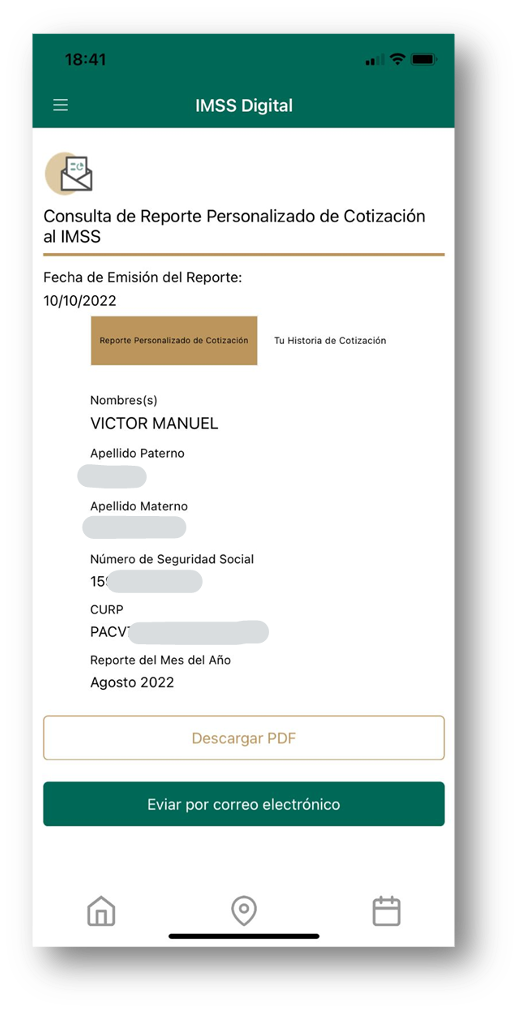
\includegraphics[width=\textwidth]{04_Figures/rpci_app/rpci_2.png}
    \end{subfigure}
    \begin{subfigure}{0.49\textwidth}
    \caption{RPCI PDF file}
    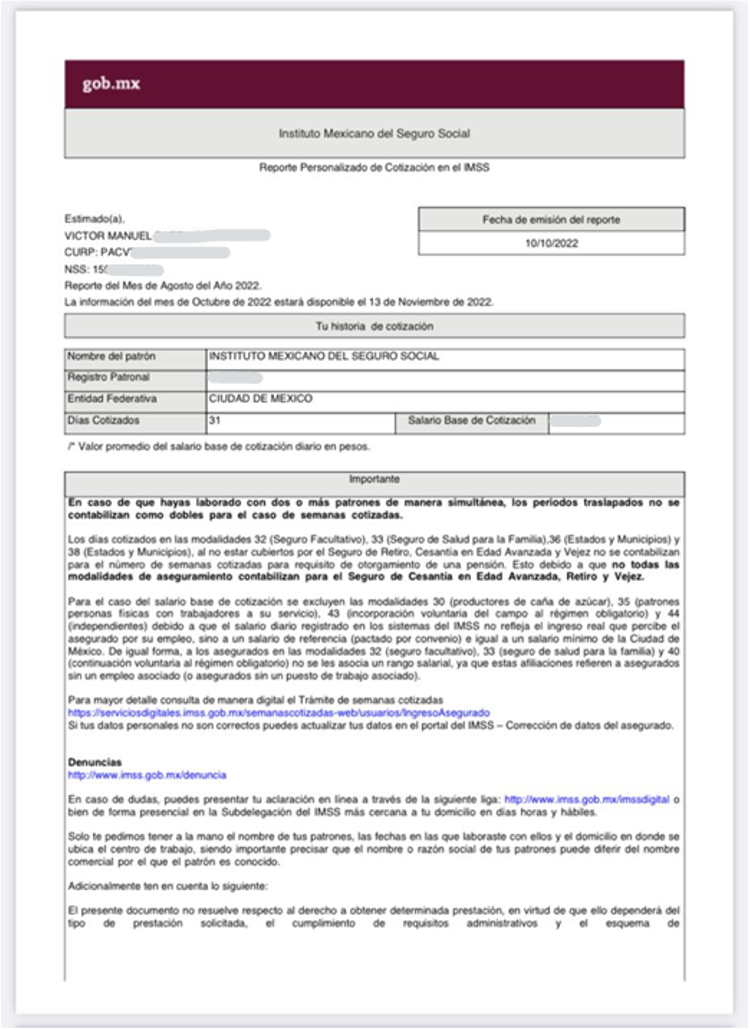
\includegraphics[width=\textwidth]{04_Figures/rpci_app/rpci_3.png}
    \end{subfigure}
    

    \end{center}
\end{figure}
\scriptsize{
\noindent Figure (a) shows the IMSS Digital app, where once the worker is registered for the RPCI, the worker can download their report in PDF or receive it via email. Figure (b) shows an example of the PDF for the RPCI. The report includes the worker job registered information, such as wage and the firm the worker is registered at.
} \\

\normalsize

We conducted an online survey of workers enrolled at IMSS in August 2021. The survey was sent via email to a random sample of workers. Figure \ref{fig:hist_knowledge_register_survey} shows the answers to some of the survey questions, related to knowledge about IMSS and wage reporting to the IMSS. This survey and our findings serve as motivation for this paper. \\

\begin{figure}[H]
    \centering
    \caption{Knowledge about IMSS and worker's reported wages \label{fig:hist_knowledge_register_survey}}
    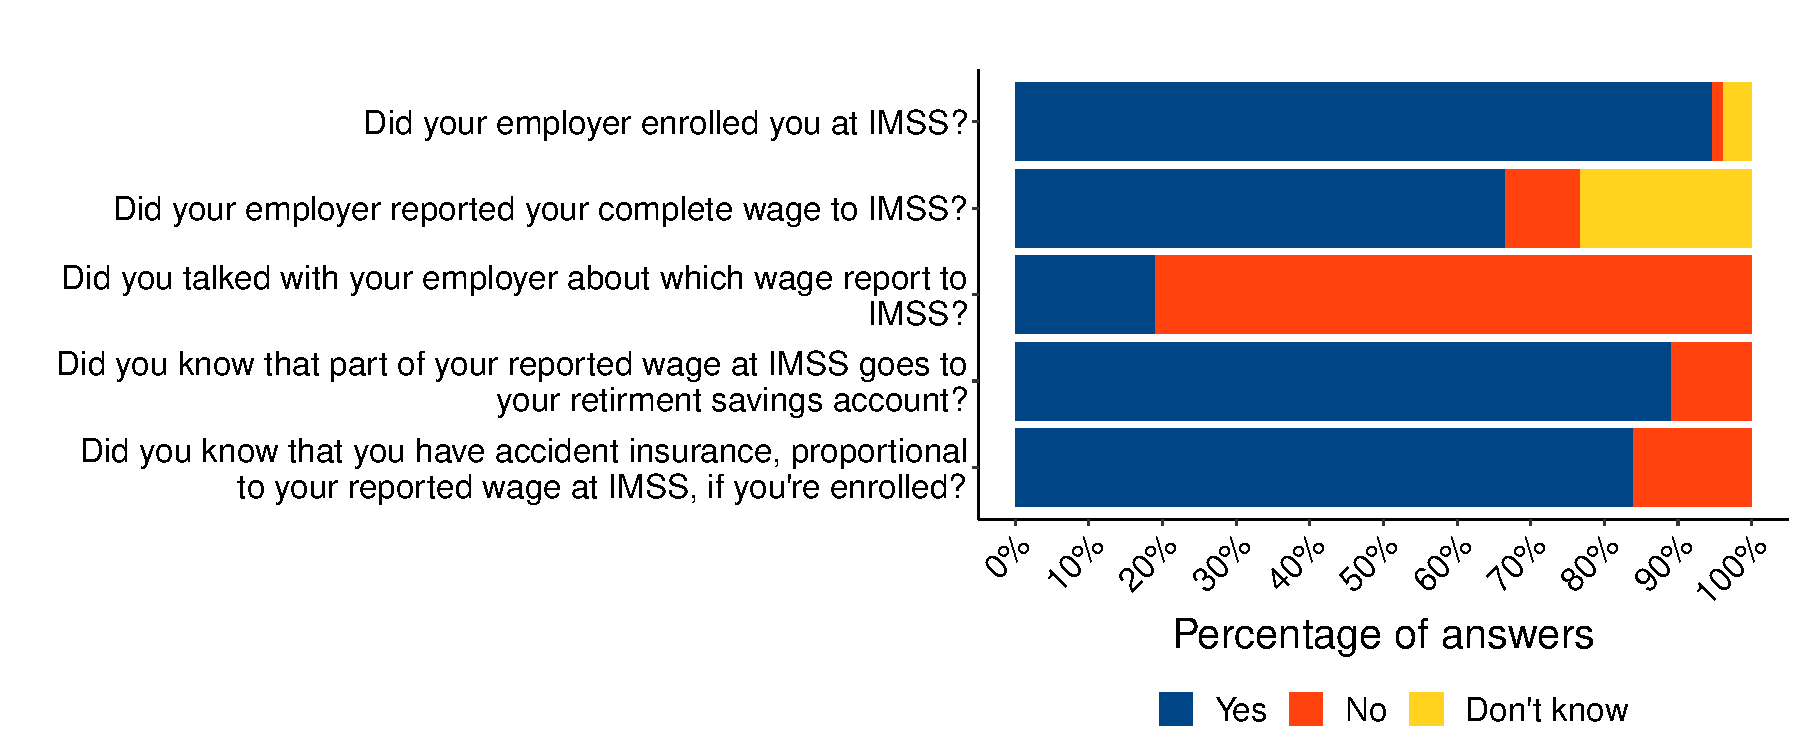
\includegraphics[width=\textwidth]{04_Figures/worker_survey/hist_knowledge_register_survey.pdf}
\end{figure}
\scriptsize{\textit{Notes}: This figure shows answers to questions about IMSS and wage reporting from the worker survey. \textit{Sample:} 233,709 answers from a survey conducted via email to workers enrolled at IMSS during August 2021. Questions 1-2, about the worker's employer, included the option "I don't know". Questions 3-5 ask about the worker's actions or knowledge didn't include the option "I don't know".
} \\

\normalsize

We find that not all workers know the status of their enrollment in the IMSS. Even though all workers were actually enrolled at IMSS, $1.5\%$ of workers said they weren't enrolled, and $4\%$ said they didn't know if they were enrolled. Moreover, workers don't always know their reported wage or know the existence of wage underreporting by their employer. When we asked in the survey if their employer reported their complete wage to the IMSS, $23.3\%$ answered that they didn't know, and $10.2\%$ said no. Most workers don't talk with their employers about which wage will be reported to the IMSS. $81\%$ of workers say they didn't talk with their employer about which wage to report to the IMSS. On the other hand, workers are aware that their benefits depend on the reported salary. $88.9\%$ report being aware that part of their reported wage goes to their savings accounts. $83.7\%$ report being aware of the existence of an accident insurance when being enrolled at IMSS, that is proportional to their reported wage. \\

Wage underreporting happens at different extents, and some workers are aware of its occurrence. Workers, in fact, could agree to underreport their own wage if the gains of paying fewer taxes are given to them and are more valued than the benefits obtained at the IMSS. If underreporting was part of an agreement, receiving information about my current job would not have an effect on me since I already knew this information. The survey answers don't exactly reflect this story. Most workers don't talk with their employers about their wages, and many don't know if their complete wage is reported. With this in mind, if underreporting happened, receiving information about my current job enrollment could trigger workers to force higher compliance in wage reporting from their employees.

\chapter{Data} \label{data}

For our main analysis, we use administrative data on workers' records from IMSS. We use a monthly panel dataset for a random sample of workers registered at IMSS during January 2021, one month before the RPCI launch. The dataset follows the workers from January 2018 to February 2022. It includes variables on the workers' registration, such as their wage, industry, age group, firm, job modality, and state. It also contains a variable on when the worker registers for the RPCI. We will refer to this dataset as the worker panel data. \\ 

Table \ref{tab:summary_stats_rpci} shows summary statistics for this data. We observe more than $1,400,000$ workers and $339,000$ firms. Our sample was a random sample of workers enrolled at the Mexican Institute of Social Security (IMSS) during 2020 and January $2021$, before the RPCI launch. Around $2\%$ of the workers in the sample registered for the RPCI at some point in our data. Workers in our sample were registered at IMSS $96\%$ of time in our data. $39.\%$ of them were women, $21\%$ we in an outsourcing schedule and $10\%$ were eventual workers. The average daily wage registered in our sample is $492.44$. \\

\begin{table}[H]
\footnotesize
\centering
\begin{threeparttable}
\centering
\caption{Summary Statistics\label{tab:summary_stats_rpci}}
%\textit{Do file: summary_stats_rpci.do}

\begin{tabular}[t]{@{}l}
\toprule
\toprule
\begin{tabular}[t]{lccc}
\input 03_Tables/muestra_10porciento/summary_stats_rpci
\midrule
Workers & & & 1,412,210\\
Firms & & & 339,884\\
\end{tabular}

\tabularnewline 
\bottomrule
\bottomrule

\end{tabular}

\begin{tablenotes}
\setlength\labelsep{0pt}
\scriptsize
\item \textit{Notes}: This table shows summary statistics on selected variables for our final sample. \textit{Sample:} Panel data for a random sample of the workers enrolled at the Mexican Institute of Social Security (IMSS) during 2020 and January 2021 (before the RPCI launch). \textit{Registered for RPCI} is a dummy where 1 means worker $i$ registered for the RPCI at some point in our sample. \textit{Enrolled} is a dummy variable where 1 means worker $i$ was enrolled at IMSS during period $t$. \textit{Women}, \textit{Outsourcing} and \textit{Eventual} are dummies where 1 means worker $i$ is a woman, an outsourced worker or an eventual worker, respectively. \textit{Wage} is registered wage for worker $i$ during period $t$. \textit{N} is the number of non-missing observations for each variable. Wage and worker characteristics are only available if the worker was registered during period $t$. \textit{Workers} and \textit{Firms} are the number of unique workers and firms in our sample. %This table is referenced in \hyperref[subsec:workers]{Section} \ref{subsec:workers}.
\end{tablenotes}
\end{threeparttable}
\end{table} \\

Workers have registered for the RPCI since it was launched in February 2021. Figure \ref{hist_download} shows the number of registers per month since the RPCI was launched. Each download month is considered a cohort for terms of the analysis in this work. Once workers register for the RPCI, they receive the report each month, in the IMSS app or via email. This creates a staggered design we can exploit. More on, not all workers registered at IMSS have registred for the RPCI, which means there exists a pure control group to compare each treatment cohort to. 

\begin{figure}[H]
    \caption{RPCI registers by month}
    \label{hist_download}
    \begin{center}
    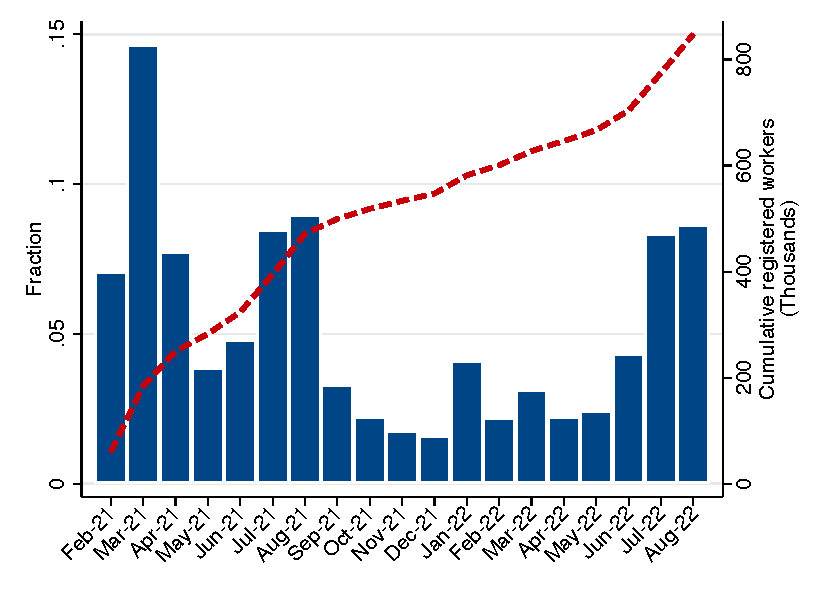
\includegraphics[width=0.65\textwidth]{04_Figures/muestra_1porciento/hist_download_month.pdf}
    \end{center}
\end{figure}
\scriptsize{
\noindent This figure shows the total number of workers registered for the RPCI. The right y-axis measures the fraction of workers who registered for the RPCI during each month from the total workers who registered for the RPCI. The left y-axis measures the cumulative number of workers who registered for the RPCI.
} \\

\normalsize

Apart from the administrative data, we have data obtained through a survey we conducted via email with IMSS. The survey received 233,709 responses from workers who answered the survey. The survey included questions on the wage the worker earns and the wage the worker thinks is registered at IMSS. It also includes questions to test the worker's level of knowledge about IMSS. This allows us to investigate the level of knowledge workers have about their reported wages. We will refer to this dataset as the survey data. This is the data where the information for Figure \ref{fig:hist_knowledge_register_survey} comes from.

\chapter{Specification} \label{specification}

Our main analysis is conducted using panel data. The treatment in our context is registration for the RPCI, which follows a staggered treatment design. Workers have the option to register for the RPCI at any time after its launch, and they can access their personalized reports on a monthly basis following registration. Consequently, we observe treatment cohorts for each month since the launch of RPCI. Moreover, not all workers registered at IMSS have enrolled in the RPCI, creating a pure control group for comparison with each treatment cohort when using causal inference methods. \\

To evaluate the causal treatment effect of registering for the RPCI, we employ a difference-in-difference (DID) analysis. Initially, we utilize a simple two-way fixed effects (TWFE) specification. However, recent literature (\citealt{de2020two}; \citealt{callaway2021difference}; \citealt{sun2021estimating}) has highlighted that TWFE estimates can be misleading or biased due to the weighted average of average treatment effects (ATEs) when negative weights or non-rare forbidden comparisons are involved, especially in cases with heterogeneous treatment effects across different treatment cohorts over time. Several authors have proposed alternative specifications to address this issue. Consequently, we also employ the specification proposed by \cite{de2020two}, incorporating the robust dynamic option to account for potential heterogeneous treatment effects across cohorts.\footnote{The estimators proposed by \cite{callaway2021difference} and \cite{sun2021estimating} are computationally challenging to implement with large samples like ours, as they involve calculating 2x2 differences between individuals and periods. \cite{de2020two} can be optimized to handle large samples, which is why we selected this estimator from among those proposed by the recent literature.}  \\

\section{Difference-in-Differences}

With two groups and two periods, a difference in differences (DID) estimator compares the outcome evolution from period 1 to 2 between a treatment group $t$ that switches from untreated to treated, and a control group $c$ that is untreated at both dates: \\

$$\text{DID} = Y_{T,2} - Y_{T,1} - (Y_{C,2} - Y_{C,1})$$

DID relies on a parallel trends assumption. In the absence of the treatment, both groups would have experienced the same outcome evolution. Specifically, for every group $g \in \{T, C\}$ and period $t \in \{1, 2\}$, let $Y_{g,t(0)}$ and $Y_{g,t(1)}$ denote the potential outcomes in group $g$ at period $t$ without and with the treatment, respectively. Parallel trends require that the expected evolution of the untreated outcome be the same in both groups. \\

\textbf{Assumption: Parallel Trends.} The expected evolution of the untreated outcome is the same in both groups: 

$$ \mathbb{E}[Y_{T,2(0)} - Y_{T,1(0)}] = \mathbb{E}[Y_{C,2(0)} - Y_{C,1(0)}]$$

Under that assumption, DID is unbiased for the average treatment effect (ATE) for the treated group at period 2 \citep{abadie2005semiparametric}:  

\begin{equation}
\begin{aligned}
\mathbb{E}[\text{DID}] &= \mathbb{E}[Y_{s,2} - Y_{s,1} - (Y_{n,2} - Y_{n,1})] \\
&= \mathbb{E}[Y_{s,2}(1) - Y_{s,1}(0) - (Y_{n,2}(0) - Y_{n,1}(0))] \\
&= \mathbb{E}[Y_{s,2}(1) - Y_{s,2}(0)] + \mathbb{E}[Y_{s,2}(0) - Y_{s,1}(0)] - \mathbb{E}[Y_{n,2}(0) - Y_{n,1}(0)] \\
&= \mathbb{E}[Y_{s,2}(1) - Y_{s,2}(0)]
\end{aligned}
\end{equation}

where the last equality follows from the parallel trends assumption. Parallel trends assumption is partly testable, by comparing the outcome trends of groups $T$ and $C$ before group $T$ received the treatment. In practice, such pre-trend tests sometimes fail, but other times they indicate that the two groups were indeed on parallel paths before $T$ got treated. \\

Motivated by the fact that in the two-groups and two-periods design described above, DID is equal to the treatment coefficient in a two-way fixed effects (TWFE) regression with group and period fixed effects, researchers have also estimated TWFE regressions in more complicated designs with many groups and periods, variation in treatment timing, treatments switching on and off, and/or non-binary treatments. Recent research has shown that in those more complicated designs, TWFE estimators are unbiased for an ATE if parallel trends hold, and if another assumption is satisfied: the treatment effect should be constant, between groups and over time. Unlike parallel trends, this assumption is unlikely to hold, even approximately, in most of the applications where TWFE regressions have been used. \\

In practice, the TWFE idea is implemented by regressing $Y_{g,t}$, the outcome in group $g$ and at period $t$, on group fixed effects, period fixed effects, and $D_{g,t}$, the treatment of group $g$ at period $t$. Such two-way fixed effects regressions are probably the most commonly used technique in economics to measure the effect of a treatment on an outcome. Researchers have long thought that TWFE estimators are equivalent to differences-in-differences (DID) estimators, but recent research has shown it isn't. \\

\subsection{Causal parameter of interest}

As in any difference-in-differences research design, I will be able to identify the Average Treatment Effect on the Treated provided that my identification assumptions hold. Consider a potential outcomes framework as introduced in \cite{Rubin} and, following the notation used in \cite{deChaisemartin_twfe_weight}, let $D_{igt}=\{0,1\}$ denote treatment status of municipality $i \in \{1, 2 , \dots, I\}$, treatment-group $g \in \{1, 2, \dots, G\}$ and time period $t \in \{1, 2, \dots, T\}$ and $Y_{igt}(D_{igt})$ denote the potential outcome of municipality $i$, treatment-group $g$ and time period $t$ as a function of the treatment $D$. Then let
\begin{equation}
    \tag{ATT_{gt}}
    \Delta_{gt} = \frac{1}{N_{gt}} \sum_{i=1}^{N_{gt}} [Y_{igt}(1) - Y_{igt}(0)]
\end{equation}
denote the Average Treatment Effect in the cell for treatment-implementation group $g$ at time period $t$. Note that
\begin{equation}
    \tag{ATT}
    \delta^{SP} = \mathbb{E}\left[\sum_{gt:D_{gt}=1} \frac{N_{gt}}{N_1} \Delta_{gt}\right]
\end{equation}
is the Average Treatment Effect on Treated municipalities ---my causal parameter of interest---, where $N_1 = \sum_{igt} D_{igt}$ is the number of treated units. The estimates for this parameter are shown in tables, whereas estimates for $ATT_{gt}$'s are shown in figures for ease of presentation.

\subsection{Estimator and identification assumptions}

For properly defining the estimator, let
\begin{equation*}
    N_{d,d^{'},t} = \sum_{g:D_{gt}=d, D_{g,t-1} = d^{'}} N_{gt} \quad \forall t \in \{2, 3, \dots, T\} \quad \forall (d, d^{'}) \in \{0,1\}^2
\end{equation*}
denote the number of observations with treatment $d^{'}$ at period $t-1$ and treatment $d$ at period $t$.  
We can now define
\begin{align*}
    DID_{+,t} = & \sum_{g:D_{gt}=1, D_{g,t-1} = 0} \frac{N_{gt}}{N_{1,0,t}} (Y_{gt} - Y_{gt-1}) - \sum_{g:D_{gt}=D_{g,t-1}=0} \frac{N_{gt}}{N_{0,0,t}} (Y_{gt} - Y_{gt-1}) \\
    DID_{-,t} = & \sum_{g:D_{gt}=D_{g,t-1} = 1} \frac{N_{gt}}{N_{1,1,t}} (Y_{gt} - Y_{gt-1}) - \sum_{g:D_{gt}=0,D_{g,t-1}=1} \frac{N_{gt}}{N_{0,1,t}} (Y_{gt} - Y_{gt-1})
\end{align*}

Then the estimator for $\delta^{SP}$ is:
\begin{equation*}
    DID = \sum_{t = 2}^T \left(\frac{N_{1,0,t}}{N_{switchers}} DID_{+,t} + \frac{N_{0,1,t}}{N_{switchers}} DID_{-,t}\right)
\end{equation*}
where $N_{switchers} = \sum_{gt: t\geq2, D_{gt}\neq D_{gt-1}} N_{gt}$
However, municipalities implementing SP did not ever stop implementing it during my period of study. Hence, the estimator for $\delta^{SP}$ reduces to:
\begin{equation*}
    DID = \sum_{t = 2}^T  \frac{N_{1,0,t}}{N_{switchers}} DID_{+,t}
\end{equation*}

Under the following identification assumptions, the $DID$ estimator is an unbiased and consistent estimator of the ATT parameter of interest (\cite{deChaisemartin_twfe_weight}.)

\paragraph{Assumption 1 - Balanced Panel} No group appears or disappears over time. \begin{align*}
\forall (g,t) \in \{1, 2, \dots, G\} \times \{1, 2, \dots, T\}, N_{gt} > 0
\end{align*}

\paragraph{Assumption 2 - Sharp Design} Units' treatments do not vary within each (g,t) cell.
\begin{align*}
\forall (g,t) \in \{1, 2, \dots, G\} \times \{1, 2, \dots, T\} \textit{ and } i \in \{1, 2, \dots, N_{gt}\}, D_{igt} = D_{gt}
\end{align*}

\paragraph{Assumption 3 - Strong Exogeneity} Shocks affecting group $g$'s untreated potential outcome, $Y_{gt}(0)$, are mean independent of grorup $g$'s treatment sequence. 
\begin{align*}
& \mathbb{E}[Y_{gt}(0) - Y_{gt-1}(0) \mid D_{g1}, D_{g2}, \dots, D_{gT}] = \mathbb{E}[Y_{gt}(0) - Y_{gt-1}(0)] \\
& \forall (g,t) \in \{1, 2, \dots, G\} \times \{1, 2, \dots, T\}
\end{align*}

\paragraph{Assumption 4 - Parallel Trends} The expectation of the outcome without treatment follows the same evolution over time in every group.
\begin{align*}
    \textit{For } t\geq 2 \quad \forall g \neq g^{'}, \mathbb{E}[Y_{gt}(0) - Y_{gt-1}(0)] = \mathbb{E}[Y_{g^{'}t}(0) - Y_{g^{'}t-1}(0)]
\end{align*}

\paragraph{Assumption 5 - Existence of ``Stable'' Groups} Between each pair of consecutive time periods, if there is a group of municipalities that implements SP, then there exists at least one group of municipalities that does not implement SP at both time periods.
\begin{align*}
    & \textit{If there is at least one } g \in \{1,2, \dots, G\} \textit{ such that } D_{gt-1} = 0, D_{gt} = 1,\\
    & \textit{ then there exists at least one } g^{'} \neq g, g^{'} \in \{1, 2, \dots, G\} \textit{ such that } D_{g^{'}t-1} = D_{g^{'}t} = 0
\end{align*}

\paragraph{Assumption 6 - Mean Independence between a Group's Outcome and Other Groups Treatments} Conditional on its own treatments, a group's outcomes are mean independent of other group's treatments.
\begin{align*}
&\forall g \in \{1, 2, \dots, G\} \textit{ let } \mathbf{D}_g = (D_{g1}, D_{g2}, \dots, D_{gT}), \textit{ then } \\
& \forall g, t, \mathbb{E}[Y_{gt}(0) \mid \mathbf{D}] = \mathbb{E}[Y_{gt}(0) \mid \mathbf{D}_g] \textit{ and } \mathbb{E}[Y_{gt}(1) \mid \mathbf{D}] = \mathbb{E}[Y_{gt}(1) \mid \mathbf{D}_g]
\end{align*}

The Balanced Panel, Sharp Design and Existence of ``Stable'' Groups assumptions are satisfied naturally given the data I have access to (see next section.) It is impossible to test whether the Parallel Trends assumption holds, however, I present evidence in favour of it by showing that one cannot reject that outcome evolution was similar between early- and later-implementer groups prior to SP implementation. As for the Strong Exogeneity assumption, I have no way to test whether it holds or not. Nonetheless, the untreated potential mortality rate's evolution is likely independent of treatment sequence for any particular group $g$ since the outcome is defined at the municipality level and, for example, if less healthy people decided to move towards early-implementing municipalities there would have to exist a sufficiently large change in the composition of people residing in the municipalities composing group $g$ in order for those changes in composition to reflect into my outcomes of interest. Also, the estimation is done $\pm 3$ years before/after SP implementation, a time window probably not as large as needed for big mobility phenomena to occur due to the implementation of SP. Lastly, Assumption 6 is also likely to hold since, for the mortality rates I am interested in, one could argue that SP being implemented earlier/later at other municipalities does not affect other group's outcomes. This is likely since, apart from AIDS, the causes of death in which I am interested are not contagious diseases.

\chapter{Results} \label{results}

We examine the effect of registering for the RPCI on enrollment and wages. The RPCI provides information about the worker's current enrollment at IMSS. If the worker's current job information is correct, receiving a report on it should not have an effect on their reported wage or employment status compared to those who didn't register for the RPCI. The worker panel data allows us to determine whether a worker $i$ was enrolled at IMSS during period $t$ and at what wage they were enrolled. We create a dummy variable, \textit{Enrolled}, where 1 indicates the worker was enrolled at IMSS during a given period. We also have information on the workers' reported wages, but this is conditional on them being enrolled at IMSS during a given period. If a worker is discharged, we don't observe their wage and have a missing value for this variable. If registering for the RPCI has an effect on the probability of being enrolled (the extensive margin), the effect on reported wages could be biased. To address this, we create another variable, \textit{Formal Wage}, which is well-defined for all periods. It is the same as the reported wage, except it is 0 instead of a missing value if the worker isn't enrolled at IMSS during a given period. \\

\section{Main Results}

Table \ref{tab:dcdh_rpci} presents the estimates obtained with a simple TWFE specification and with the \cite{de2020two} specification. We find no effect on the probability of being enrolled at IMSS. We observe a positive and significant treatment effect of registering for the RPCI on the reported wage and formal wage using the TWFE estimate, but no significant effect on formal wages when looking into the \cite{de2020two} estimate. This is mainly due to the imputation of zeros to formal wages, which would lower the average treatment effect found in the reported wage. A more comprehensive way of addressing this would be imputating another value, say the value of their wage when they are informal workers, but this is an unobservable value. \\

\begin{table}[H]
\footnotesize
\centering
\begin{threeparttable}
\centering
\caption{RPCI effect on enrollment and wages\label{tab:dcdh_rpci}}
%\textit{Do file: event_study_rpci.do}

\begin{tabularx}{\textwidth}[t]{@{}l@{}l@{}l@{}l}
\toprule
\toprule
\multicolumn{4}{c}{\textit{Panel A:} TWFE} \\
\midrule
\begin{tabular}[t]{p{0.2\textwidth}P{0.15\textwidth}}
& Enrolled \\
\midrule
\input 03_Tables/muestra_10porciento/twfe_alta_wo_extended
\end{tabular}
&
\begin{tabular}[t]{HP{0.15\textwidth}}
& Formal Wage$^\dagger$ \\
\midrule
\input 03_Tables/muestra_10porciento/twfe_sal_formal_wo_extended
\end{tabular}
&
\begin{tabular}[t]{HP{0.15\textwidth}}
& Wage \\
\midrule
\input 03_Tables/muestra_10porciento/twfe_sal_cierre_wo_extended
\end{tabular}
&
\begin{tabular}[t]{HP{0.15\textwidth}}
& Log Wage \\
\midrule
\input 03_Tables/muestra_10porciento/twfe_log_sal_cierre_wo_extended
\end{tabular}
\end{tabularx}

\begin{tabularx}{\textwidth}[t]{@{}l@{}l@{}l@{}l}
\toprule
\toprule
\multicolumn{4}{c}{\textit{Panel B:} \cite{de2020two}} \\
\midrule
\begin{tabular}[t]{p{0.2\textwidth}P{0.15\textwidth}}
& Enrolled \\
\midrule
\input 03_Tables/muestra_10porciento/dcdh_alta
\end{tabular}
&
\begin{tabular}[t]{HP{0.15\textwidth}}
& Formal Wage$^\dagger$ \\
\midrule
\input 03_Tables/muestra_10porciento/dcdh_sal_formal
\end{tabular}
&
\begin{tabular}[t]{HP{0.15\textwidth}}
& Wage \\
\midrule
\input 03_Tables/muestra_10porciento/dcdh_sal_cierre
\end{tabular}
&
\begin{tabular}[t]{HP{0.15\textwidth}}
& Log Wage \\
\midrule
\input 03_Tables/muestra_10porciento/dcdh_log_sal_cierre
\end{tabular}

\tabularnewline 
\bottomrule
\bottomrule

\end{tabularx}

\begin{tablenotes}
\setlength\labelsep{0pt}
\scriptsize
\item \textit{Notes}: This table shows the effect of registering to the RPCI on enrollment and the worker's wage. \textit{Sample:} Panel data for a random sample of the workers enrolled at the Mexican Institute of Social Security (IMSS) during 2020 and January 2021 (before the RPCI launch). \textit{Enrolled} is a dummy variable where 1 means worker $i$ was enrolled at IMSS during period $t$. $\dagger$ \textit{Formal Wage} and \textit{Wage} are the registered wage for worker $i$ during period $t$, the difference is \textit{Formal Wage} is 0 when the worker isn't enrolled, while \textit{Wage} is missing when the worker isn't enrolled. \textit{Panel A} displays the coefficients obtained from simple TWFE specifications. \textit{Panel B} displays the average treatment effect estimated following \cite{de2020two}, using the robust dynamic option to account for possible heterogeneous treatment effects across cohorts. The number of observations in \textit{Panel B} is the number of differences between the outcome and the treatment used in the estimation. The effect is the average effect of the treatment across the switchers. Switchers are the number of switchers this effect applies to. Robust standard errors clustered by worker id in parenthesis. *** $p<0.01$, ** $p<0.05$, * $p<0.1$. %This table is referenced in %\hyperref[subsec:workers]{Section} \ref{subsec:workers}.
\end{tablenotes}
\end{threeparttable}
\end{table}

Figure \ref{fig:event_study_rpci} presents the event studies using the simple TWFE specification and the \cite{de2020two} specification. The event study shows no differences between treated and control groups before registering for the RPCI. The event studies show a positive effect of registering for the RPCI on the worker's registered wage. More on, Table \ref{tab:dcdh_rpci} shows an effect on wages of approximately $1.5\%-2\%$ of the daily average wage ($\$496$). The event studies also show the effect is increasing, so the table estimate is the average across the dynamic effects. The wage event studies show an effect of approximately $4\%$ of the daily average wage 12 months after registering for the RPCI ($\$20$). \\


\begin{figure}[H]
    \centering
    \caption{Event studies - RPCI effect on enrollment and wages \label{fig:event_study_rpci}}
    
    \begin{subfigure}{0.49\textwidth}
    \caption{Effect on being enrolled}
    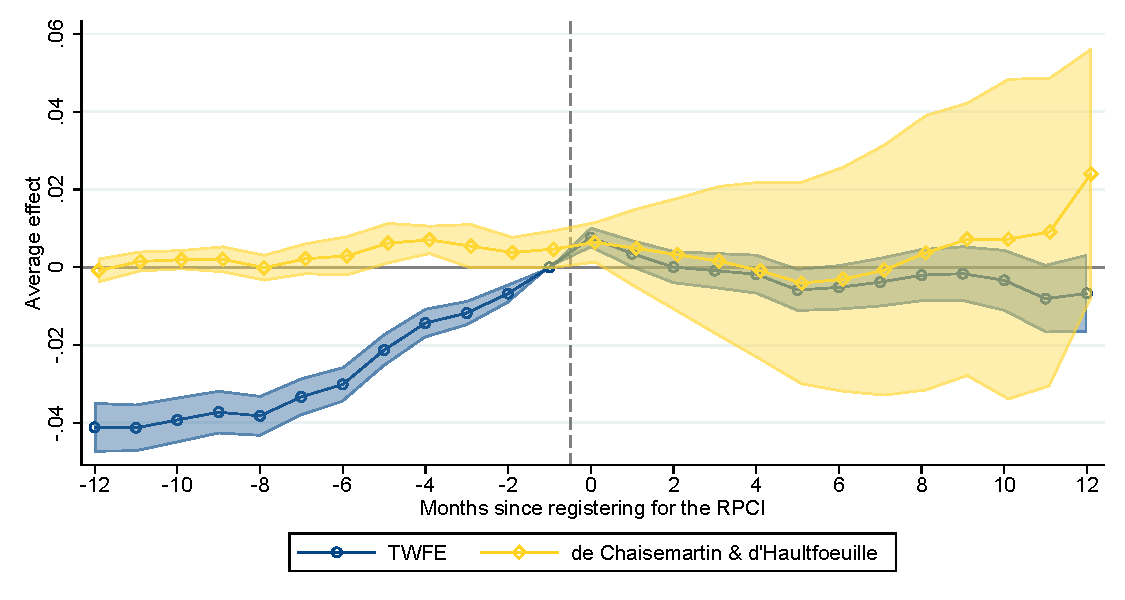
\includegraphics[width=\textwidth]{04_Figures/muestra_10porciento/event_study_alta_connected.pdf}
    \end{subfigure}
    \begin{subfigure}{0.49\textwidth}
    \caption{Effect on formal wage$^\dagger$}
    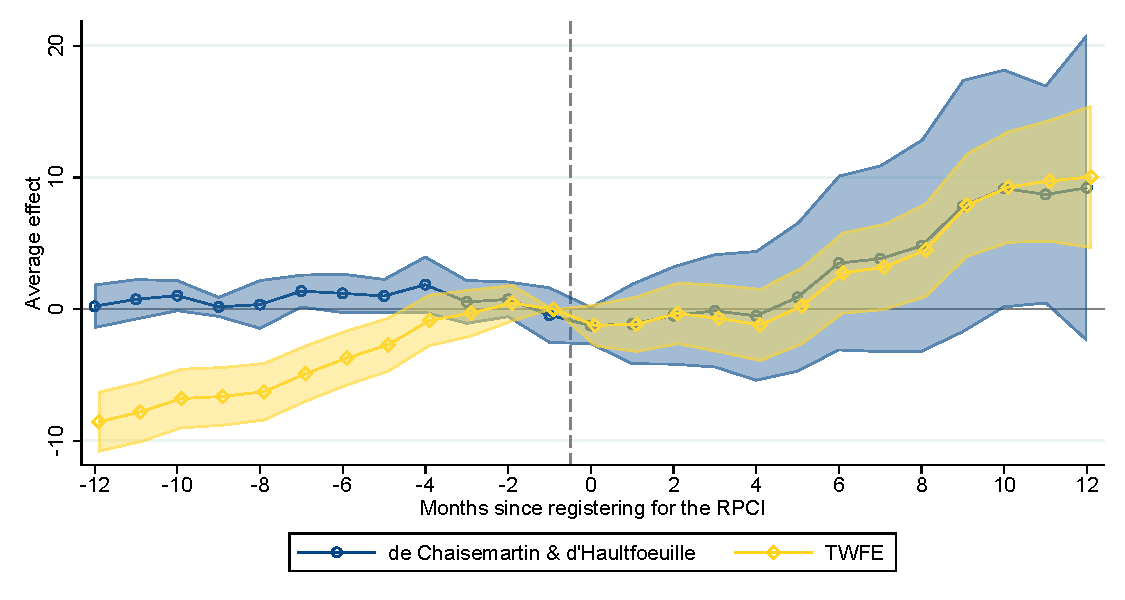
\includegraphics[width=\textwidth]{04_Figures/muestra_10porciento/event_study_sal_formal_connected.pdf}
    \end{subfigure}
    
    \begin{subfigure}{0.49\textwidth}
    \caption{Effect on wage}
    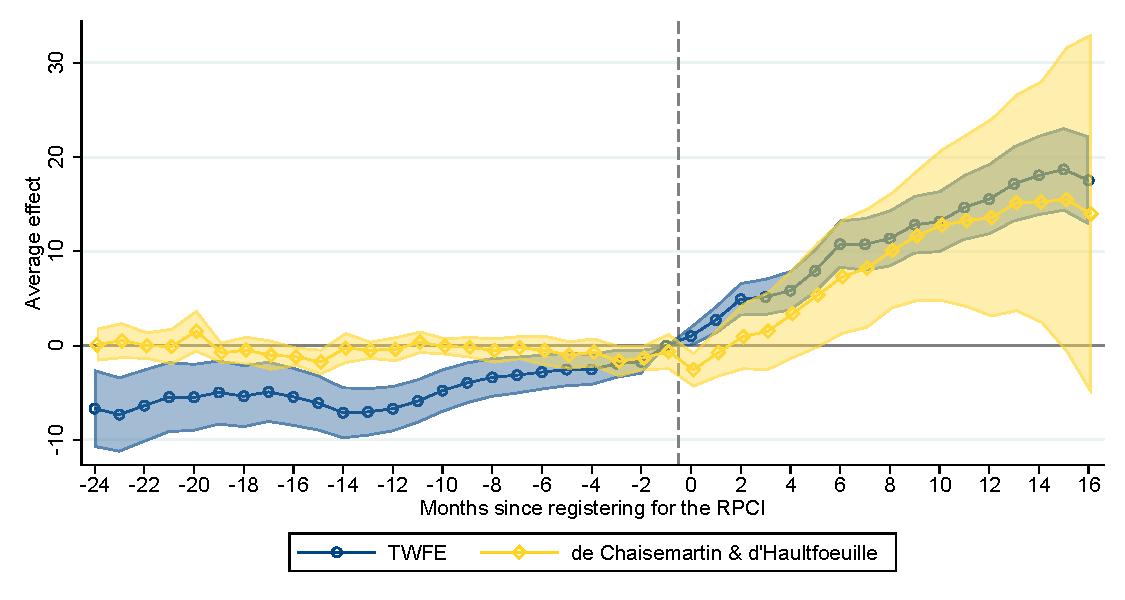
\includegraphics[width=\textwidth]{04_Figures/muestra_10porciento/event_study_sal_cierre_connected.pdf}
    \end{subfigure}
    \begin{subfigure}{0.49\textwidth}
    \caption{Effect on log wage}
    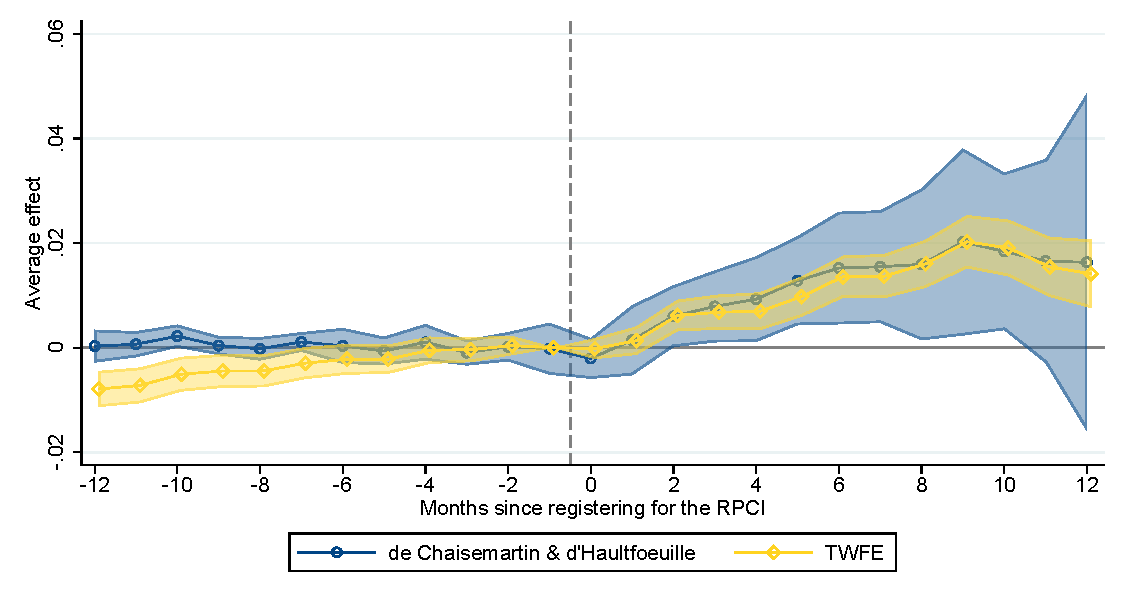
\includegraphics[width=\textwidth]{04_Figures/muestra_10porciento/event_study_log_sal_cierre_connected.pdf}
    \end{subfigure}
    
    %\textit{Do file: event_study_rpci.do}
\end{figure}

\scriptsize{
\noindent \textit{Notes}: This figure shows the event studies for the effect of registering to the RPCI on enrollment and the worker's wage. \textit{Sample:} Panel data for a random sample of the workers enrolled at the Mexican Institute of Social Security (IMSS) during 2020 and January 2021 (before the RPCI launch). \textit{Enrolled} is a dummy variable where 1 means worker $i$ was enrolled at IMSS during period $t$. $\dagger$ \textit{Formal Wage} and \textit{Wage} are the registered wage for worker $i$ during period $t$, the difference is \textit{Formal Wage} is 0 when the worker isn't enrolled, while \textit{Wage} is missing when the worker isn't enrolled. The lighter-shaded event studies present the estimators obtained from a TWFE specification. The darker-shaded event studies follow the estimators proposed by \cite{de2020two}, using the robust dynamic option to account for possible heterogeneous treatment effects across cohorts. Robust standard errors clustered by worker id. %This figure is referenced in \hyperref[subsec:workers]{Section} \ref{subsec:workers}.
} \\

\normalsize

\section{Heterogeneity by worker characteristics}

We also investigate the heterogeneity of treatment effects by worker and firm characteristics at baseline. Figure \ref{fig:heterogeneity_worker_rpci} shows the resulting estimated coefficients by worker characteristics using the \cite{de2020two} specification. When examining gender, we can observe a higher treatment effect on men's wages, but a higher effect on women's log wages. This is consistent with the fact that women have lower wages than men, so even if the effect in terms of pesos is lower, relative to their wages the effect could be proportionally higher. Young workers (25-35 years) have a significant positive treatment on formal wages, and a significant effect on wages and log wages at a 10\% significance level. Older workers near retirement age (65 years) have interesting treatment effects: a negative treatment effect on the probability of being enrolled, a negative treatment effect on formal wages, but a positive treatment effect on reported wages. These results could indicate that older workers have a make-or-break negotiation with their employers when they find out their actual reported wage to IMSS, as their pension and retirement savings depend on the reported wage. We also observe a positive treatment effect for workers earning between 1 and 2 minimum wages and those earning between 2 and 3 minimum wages, while there is no effect for those with higher wages. This is consistent with firms registering workers to IMSS with just the minimum possible wage or just a bit above the minimum wage, as we can see the highest effect on log wages is for workers that earn between 1 and 2 minimum wages at baseline. The event studies for this estimates are shown in the Appendix. \\

\begin{figure}[H]
    \centering
    \caption{Heterogeneity by worker characteristics \label{fig:heterogeneity_worker_rpci}}
    
    \begin{subfigure}{\textwidth}
    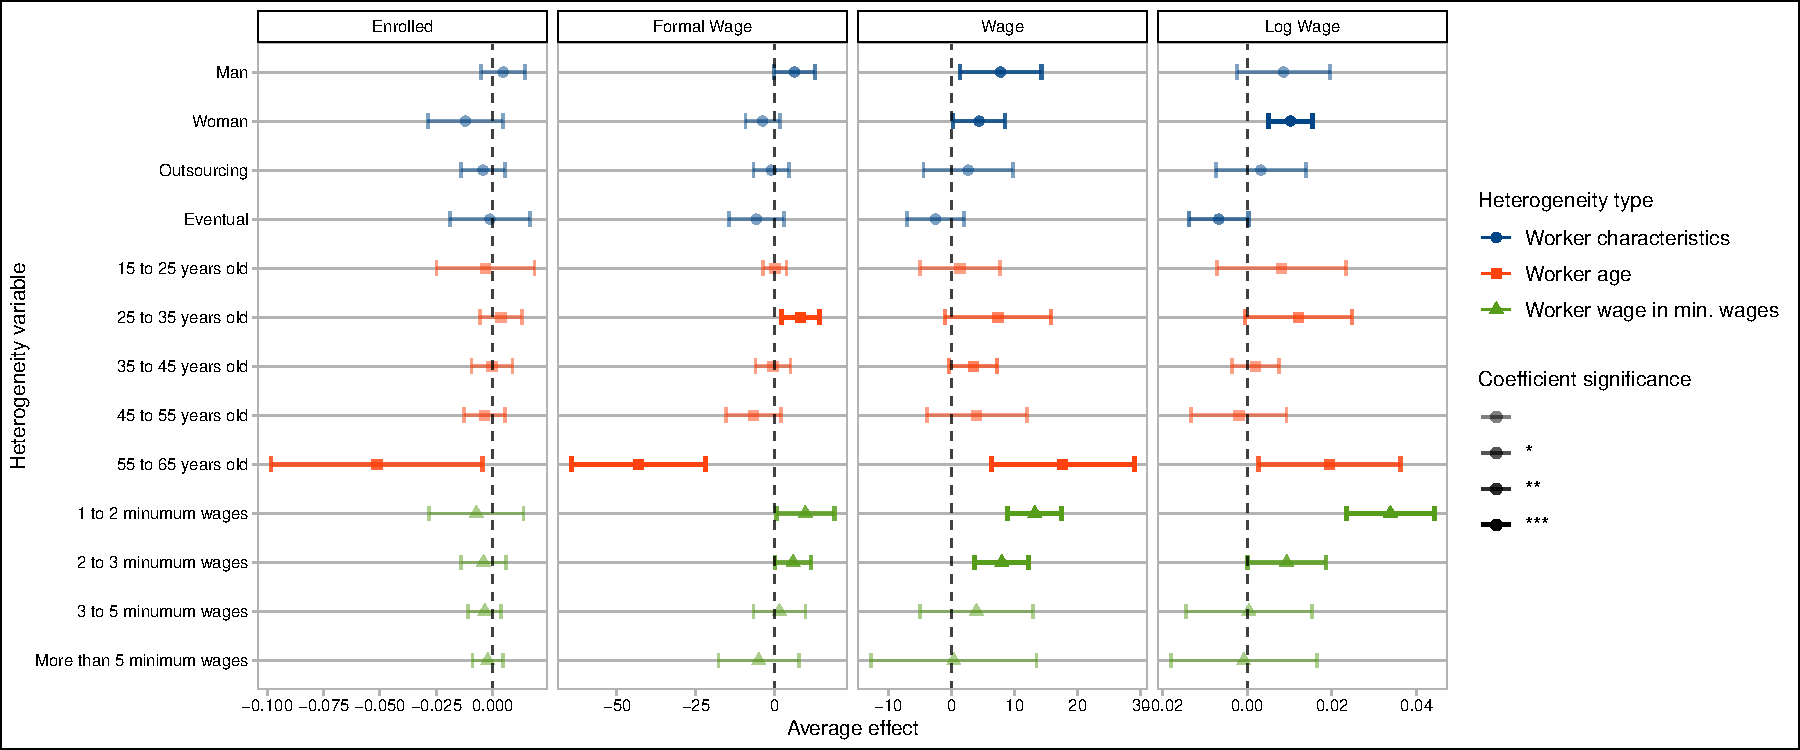
\includegraphics[width=\textwidth]{04_Figures/muestra_10porciento/dcdh_heterogeneity_worker_characteristics.pdf}
    \end{subfigure}
    
    %\textit{Do file: dcdh_heterogeneity_rpci.do}
\end{figure}

\scriptsize{
\noindent \textit{Notes}: This figure explores heterogeneity in the effect of registering to the RPCI on enrollment and the worker's wage by baseline worker's characteristics (characteristics during 2020, before the RPCI launch). \textit{Sample:} Panel data for a random sample of the workers enrolled at the Mexican Institute of Social Security (IMSS) during 2020 and January 2021 (before the RPCI launch). \textit{Enrolled} is a dummy variable where 1 means worker $i$ was enrolled at IMSS during period $t$. $\dagger$ \textit{Formal Wage} and \textit{Wage} are the registered wage for worker $i$ during period $t$, the difference is \textit{Formal Wage} is 0 when the worker isn't enrolled, while \textit{Wage} is missing when the worker isn't enrolled. The coefficient displayed is the average treatment effect estimated following \cite{de2020two}, using the robust dynamic option to account for possible heterogeneous treatment effects across cohorts. 95\% confidence intervals are shown. Robust standard errors clustered by worker id. *** $p<0.01$, ** $p<0.05$, * $p<0.1$. %This figure is referenced in %\hyperref[subsec:workers]{Section} \ref{subsec:workers}.
} \\

\normalsize

\section{Heterogeneity by firm characteristics}

Figure \ref{fig:heterogeneity_firm_rpci} shows the resulting estimated coefficients by firm characteristics. Job registers at IMSS have a municipality identifier when they are permanent jobs registered by a firm. We examine the treatment effect for workers in the MX-USA border and workers away from the border. We use INEGI's definition of border municipalities, which is the same as that used to establish differentiated minimum wages between the border and the rest of the country. We find a positive treatment effect on wages for both workers along the border and away from the border, with a higher point estimate along the border, although not statistically different from the estimate away from the border. The fact that both are significant could be more a proxy of a significant effect on permanent jobs registered at IMSS. By region, we find a positive treatment effect on wages in the Central-West and North region, with the effect being higher for the former. By firm industry, we find positive treatment effects on wages in the agriculture, construction, and services industries, with construction having the highest effect on log wages. By firm size, we find a positive treatment effect on small firms (2-5 workers) and medium firms (6-50 and 51-250 workers), which is consistent with previous research that finds the a negative relation between underreporting and firm size. The event studies for this estimates are shown in the Appendix. \\

\begin{figure}[H]
    \centering
    \caption{Heterogeneity by firm characteristics \label{fig:heterogeneity_firm_rpci}}
    
    \begin{subfigure}{\textwidth}
    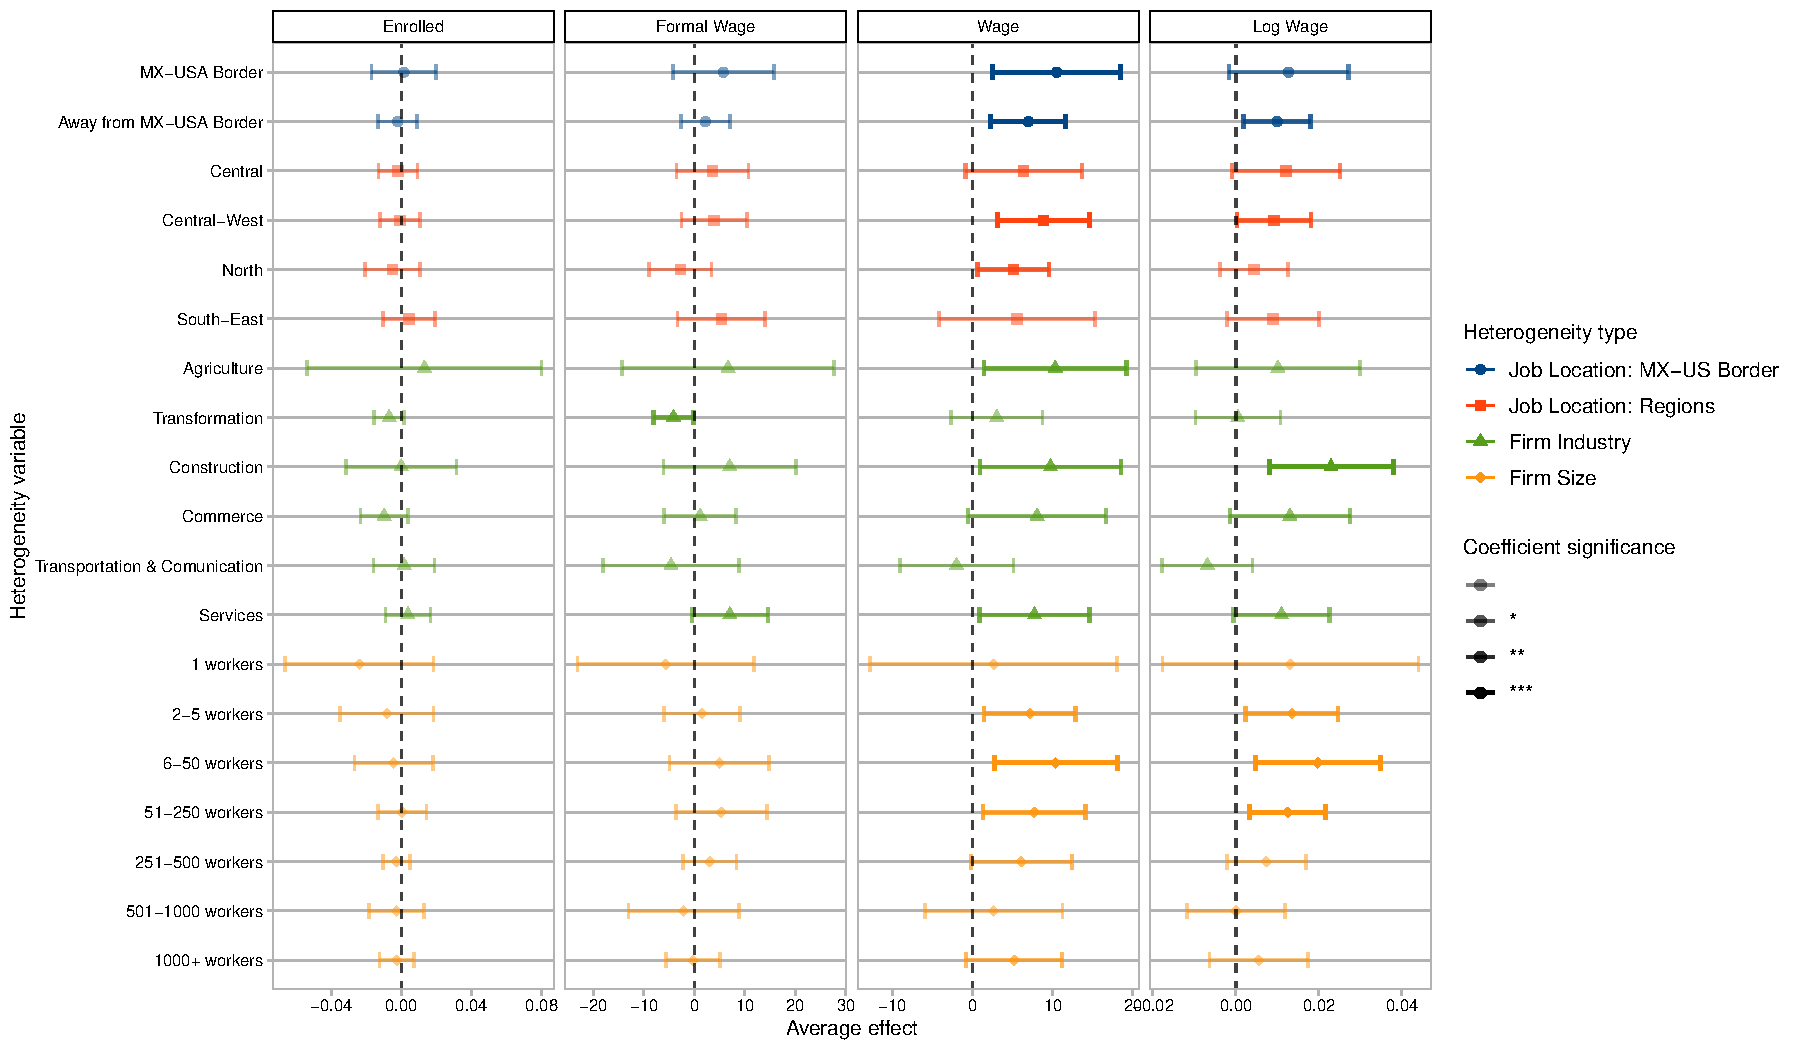
\includegraphics[width=\textwidth]{04_Figures/muestra_10porciento/dcdh_heterogeneity_firm_characteristics.pdf}
    \end{subfigure}
    
    %\textit{Do file: dcdh_heterogeneity_rpci.do}
\end{figure}

\scriptsize{
\noindent \textit{Notes}: This figure explores heterogeneity in the effect of registering to the RPCI on enrollment and the worker's wage by baseline firm's characteristics (characteristics during 2020, before the RPCI launch). \textit{Sample:} Panel data for a random sample of the workers enrolled at the Mexican Institute of Social Security (IMSS) during 2020 and January 2021 (before the RPCI launch). \textit{Enrolled} is a dummy variable where 1 means worker $i$ was enrolled at IMSS during period $t$. $\dagger$ \textit{Formal Wage} and \textit{Wage} are the registered wage for worker $i$ during period $t$, the difference is \textit{Formal Wage} is 0 when the worker isn't enrolled, while \textit{Wage} is missing when the worker isn't enrolled. The coefficient displayed is the average treatment effect estimated following \cite{de2020two}, using the robust dynamic option to account for possible heterogeneous treatment effects across cohorts. 95\% confidence intervals shown. Robust standard errors clustered by worker id. *** $p<0.01$, ** $p<0.05$, * $p<0.1$. %This figure is referenced in \hyperref[subsec:workers]{Section} \ref{subsec:workers}.
}

\normalsize

\chapter{Conclusion} \label{conclusion}

%%%%%%%%%%%%%%%%%%%%%%%%%%%%%%%%%%%%%%%%%%%%%%%%%%%%%%%%%%%%%

\newpage

%%%%%%%%%%%%%%%%%%%%%%%%%%%%%%%%%%%%%%%%%%%%%%%%%%%%%%%%%%%%%
%BIBLIOGRAPHY

\clearpage
\bibliographystyle{ecta}
%\bibliographystyle{authordate1}
%\bibliographystyle{amsalpha}
%\bibliographystyle{AEA}

\bibliography{References}

%\FloatBarrier
%%%%%%%%%%%%%%%%%%%%%%%%%%%%%%%%%%%%%%%%

\clearpage
\singlespacing

\begin{comment}

\chapter{Tables}


\begin{table}[H]
\footnotesize
\centering
\begin{threeparttable}
\centering
\caption{Summary Statistics\label{tab:summary_stats_rpci}}
%\textit{Do file: summary_stats_rpci.do}

\begin{tabular}[t]{@{}l}
\toprule
\toprule
\begin{tabular}[t]{lccc}
\input 03_Tables/muestra_10porciento/summary_stats_rpci
\midrule
Workers & & & 1,412,210\\
Firms & & & 339,884\\
\end{tabular}

\tabularnewline 
\bottomrule
\bottomrule

\end{tabular}

\begin{tablenotes}
\setlength\labelsep{0pt}
\scriptsize
\item \textit{Notes}: This table shows summary statistics on selected variables for our final sample. \textit{Sample:} Panel data for a random sample of the workers enrolled at the Mexican Institute of Social Security (IMSS) during 2020 and January 2021 (before the RPCI launch). \textit{Registered for RPCI} is a dummy where 1 means worker $i$ registered for the RPCI at some point in our sample. \textit{Enrolled} is a dummy variable where 1 means worker $i$ was enrolled at IMSS during period $t$. \textit{Women}, \textit{Outsourcing} and \textit{Eventual} are dummies where 1 means worker $i$ is a woman, an outsourced worker or an eventual worker, respectively. \textit{Wage} is registered wage for worker $i$ during period $t$. \textit{N} is the number of non-missing observations for each variable. Wage and worker characteristics are only available if the worker was registered during period $t$. \textit{Workers} and \textit{Firms} are the number of unique workers and firms in our sample. This table is referenced in %\hyperref[subsec:workers]{Section} \ref{subsec:workers}.
\end{tablenotes}
\end{threeparttable}
\end{table}

\clearpage


\begin{table}[H]
\footnotesize
\centering
\begin{threeparttable}
\centering
\caption{RPCI effect on enrollment and wages\label{tab:dcdh_rpci}}
%\textit{Do file: event_study_rpci.do}

\begin{tabularx}{\textwidth}[t]{@{}l@{}l@{}l@{}l}
\toprule
\toprule
\multicolumn{4}{c}{\textit{Panel A:} TWFE} \\
\midrule
\begin{tabular}[t]{p{0.2\textwidth}P{0.15\textwidth}}
& Enrolled \\
\midrule
\input 03_Tables/muestra_10porciento/twfe_alta_wo_extended
\end{tabular}
&
\begin{tabular}[t]{HP{0.15\textwidth}}
& Formal Wage$^\dagger$ \\
\midrule
\input 03_Tables/muestra_10porciento/twfe_sal_formal_wo_extended
\end{tabular}
&
\begin{tabular}[t]{HP{0.15\textwidth}}
& Wage \\
\midrule
\input 03_Tables/muestra_10porciento/twfe_sal_cierre_wo_extended
\end{tabular}
&
\begin{tabular}[t]{HP{0.15\textwidth}}
& Log Wage \\
\midrule
\input 03_Tables/muestra_10porciento/twfe_log_sal_cierre_wo_extended
\end{tabular}
\end{tabularx}

\begin{tabularx}{\textwidth}[t]{@{}l@{}l@{}l@{}l}
\toprule
\toprule
\multicolumn{4}{c}{\textit{Panel B:} \cite{de2020two}} \\
\midrule
\begin{tabular}[t]{p{0.2\textwidth}P{0.15\textwidth}}
& Enrolled \\
\midrule
\input 03_Tables/muestra_10porciento/dcdh_alta
\end{tabular}
&
\begin{tabular}[t]{HP{0.15\textwidth}}
& Formal Wage$^\dagger$ \\
\midrule
\input 03_Tables/muestra_10porciento/dcdh_sal_formal
\end{tabular}
&
\begin{tabular}[t]{HP{0.15\textwidth}}
& Wage \\
\midrule
\input 03_Tables/muestra_10porciento/dcdh_sal_cierre
\end{tabular}
&
\begin{tabular}[t]{HP{0.15\textwidth}}
& Log Wage \\
\midrule
\input 03_Tables/muestra_10porciento/dcdh_log_sal_cierre
\end{tabular}

\tabularnewline 
\bottomrule
\bottomrule

\end{tabularx}

\begin{tablenotes}
\setlength\labelsep{0pt}
\scriptsize
\item \textit{Notes}: This table shows the effect of registering to the RPCI on enrollment and the worker's wage. \textit{Sample:} Panel data for a random sample of the workers enrolled at the Mexican Institute of Social Security (IMSS) during 2020 and January 2021 (before the RPCI launch). \textit{Enrolled} is a dummy variable where 1 means worker $i$ was enrolled at IMSS during period $t$. $\dagger$ \textit{Formal Wage} and \textit{Wage} are the registered wage for worker $i$ during period $t$, the difference is \textit{Formal Wage} is 0 when the worker isn't enrolled, while \textit{Wage} is missing when the worker isn't enrolled. \textit{Panel A} displays the coefficients obtained from simple TWFE specifications. \textit{Panel B} displays the average treatment effect estimated following \cite{de2020two}, using the robust dynamic option to account for possible heterogeneous treatment effects across cohorts. The number of observations in \textit{Panel B} is the number of differences between the outcome and the treatment used in the estimation. The effect is the average effect of the treatment across the switchers. Switchers are the number of switchers this effect applies to. Robust standard errors clustered by worker id in parenthesis. *** $p<0.01$, ** $p<0.05$, * $p<0.1$. This table is referenced in %\hyperref[subsec:workers]{Section} \ref{subsec:workers}.
\end{tablenotes}
\end{threeparttable}
\end{table}

\clearpage


\begin{comment}
\subsection{RPCI effect on wage changes}

\begin{table}[H]
\footnotesize
\centering
\begin{threeparttable}
\centering
\caption{RPCI effect on wage changes\label{tab:dcdh_wage_changes_rpci}}
%\textit{Do file: yearly_volatility_rpci.do}

\begin{tabularx}{0.75\textwidth}[t]{@{}l@{}l@{}l}
\toprule
\toprule
\begin{tabular}[t]{p{0.2\textwidth}P{0.15\textwidth}}
& Wage Changes \\
\midrule
\input 03_Tables/muestra_10porciento/dcdh_sal_diff_yr
\end{tabular}
&
\begin{tabular}[t]{HP{0.15\textwidth}}
& Wage Raises \\
\midrule
\input 03_Tables/muestra_10porciento/dcdh_sal_mayor_yr
\end{tabular}
&
\begin{tabular}[t]{HP{0.15\textwidth}}
& Wage Cuts \\
\midrule
\input 03_Tables/muestra_10porciento/dcdh_sal_menor_yr
\end{tabular}

\tabularnewline 
\bottomrule
\bottomrule

\end{tabularx}

\begin{tablenotes}
\setlength\labelsep{0pt}
\scriptsize
\item \textit{Notes}: This table shows the effect of registering to the RPCI on wage changes per year. \textit{Sample:} Panel data for a random sample of the workers enrolled at the Mexican Institute of Social Security (IMSS) during 2020 and January 2021 (before the RPCI launch). \textit{Wage Changes} counts the number of changes in the reported wage at IMSS of worker $i$ during year $t$. \textit{Wage Raises} counts the number of wage changes where the wage increased and \textit{Wage Cuts} counts the number of wage changes where the wage decreased. The coefficient displayed is the treatment effect on the year after being treated estimated following \cite{de2020two}. The number of observations are the number of differences of the outcome and of the treatment used in the estimation. The effect is the average effect of the treatment across the switchers. Switchers is the number of switchers this effect applies to. Robust standard errors clustered by worker id in parenthesis. *** $p<0.01$, ** $p<0.05$, * $p<0.1$. This table is referenced in %\hyperref[subsec:wage_changes]{Section} \ref{subsec:wage_changes}.
\end{tablenotes}
\end{threeparttable}
\end{table}
\clearpage


\singlespacing

\chapter{Figures}

%\subsection{Knowledge about IMSS}

\vspace{.7in}
\begin{figure}[H]
    \centering
    \caption{Knowledge about IMSS and worker's reported wages \label{fig:hist_knowledge_register_survey}}
    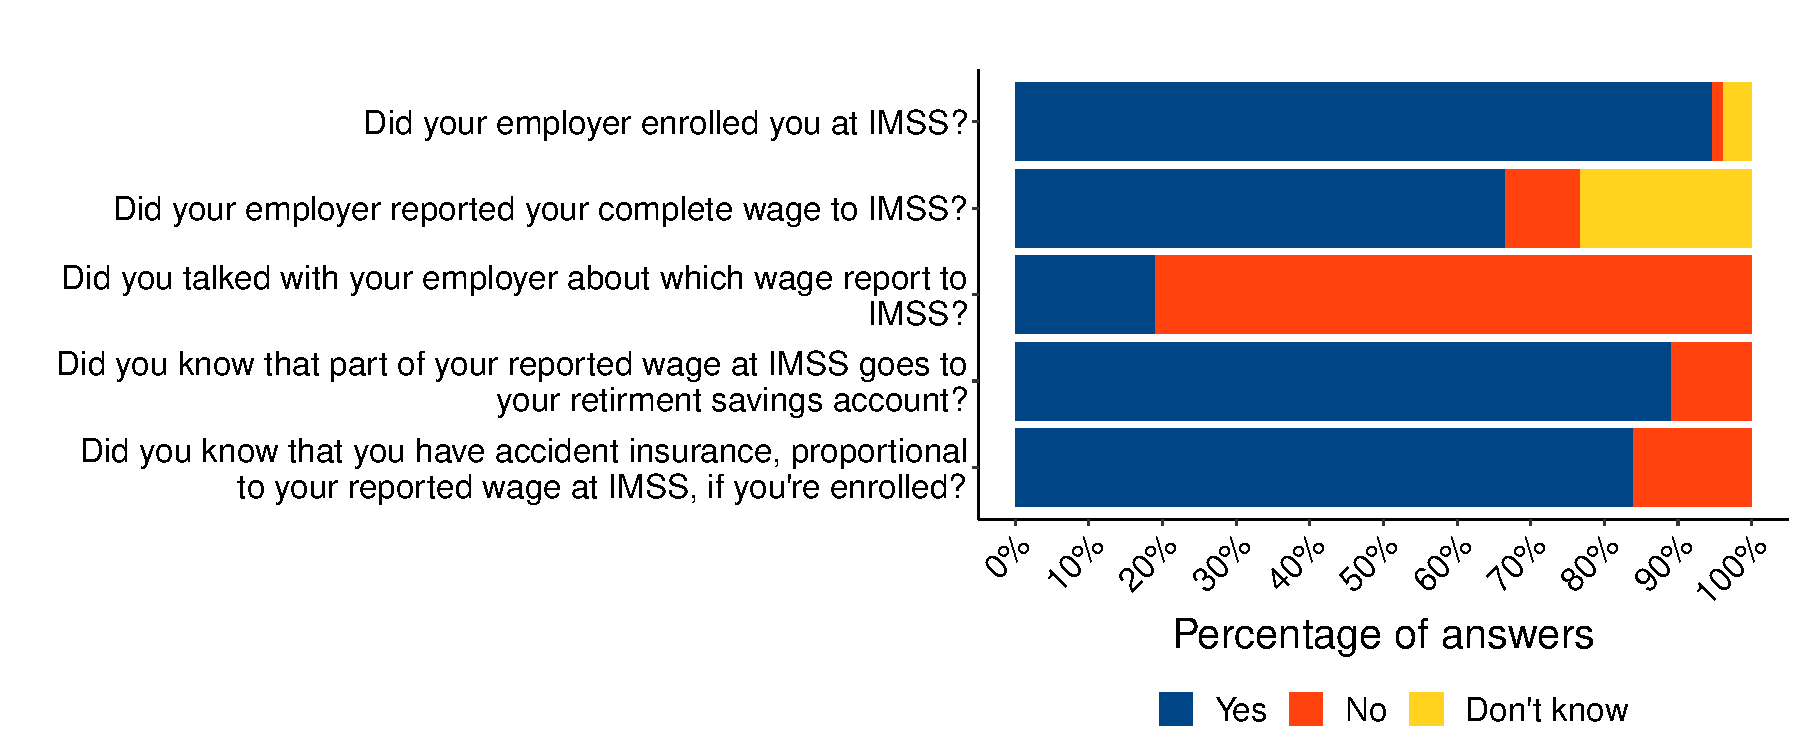
\includegraphics[width=\textwidth]{04_Figures/worker_survey/hist_knowledge_register_survey.pdf}
\end{figure}
\scriptsize{\textit{Notes}: This figure shows answers to questions about IMSS and wage reporting from the worker survey. \textit{Sample:} 233,709 answers from a survey conducted via email to workers enrolled at IMSS during August 2021. Questions 1-2, about the worker's employer, included the option "I don't know". Questions 3-5 ask about the worker's actions or knowledge didn't include the option "I don't know".}

\clearpage

%\subsection{RPCI}

\begin{figure}[H]
    \label{rpci_example}
    \caption{RPCI example}
    \begin{center}
    
    \begin{subfigure}{0.49\textwidth}
    \caption{RPCI within the IMSS Digital app}
    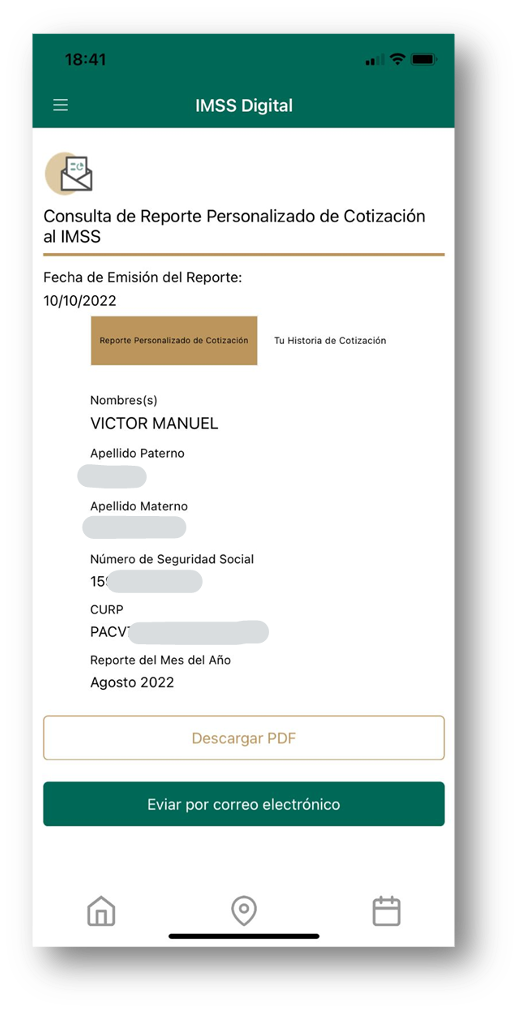
\includegraphics[width=\textwidth]{04_Figures/rpci_app/rpci_2.png}
    \end{subfigure}
    \begin{subfigure}{0.49\textwidth}
    \caption{RPCI PDF file}
    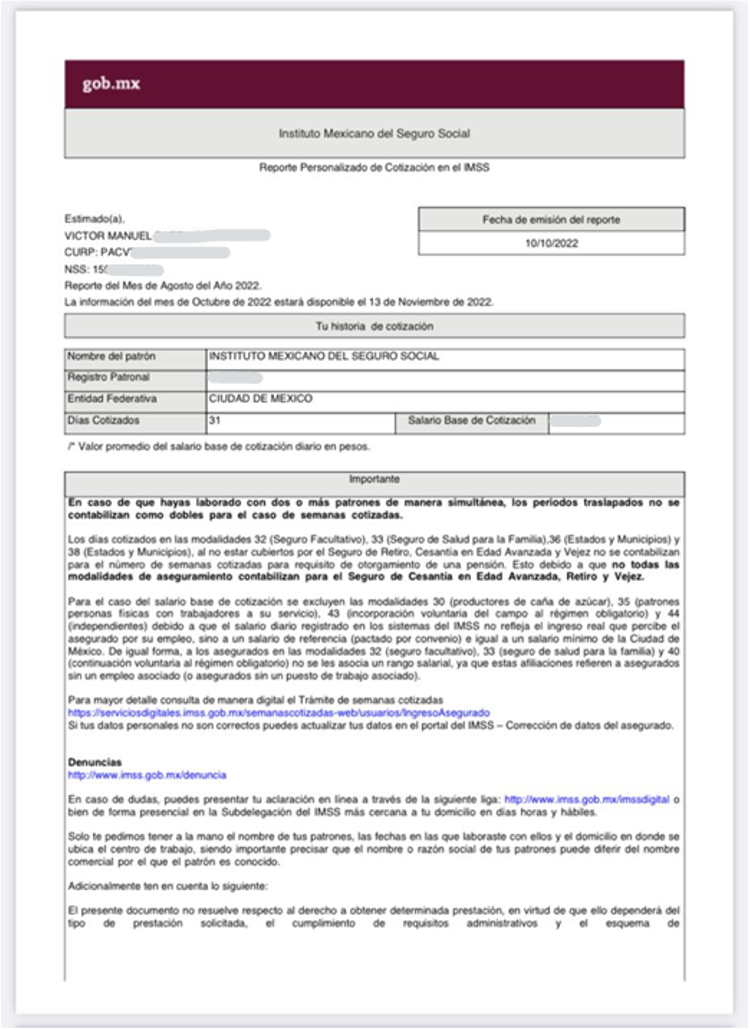
\includegraphics[width=\textwidth]{04_Figures/rpci_app/rpci_3.png}
    \end{subfigure}
    

    \end{center}
\end{figure}
\scriptsize{
\noindent Figure (a) shows the IMSS Digital app, where once the worker is registered for the RPCI, the worker can download their report in PDF or receive it via email. Figure (b) shows an example of the PDF for the RPCI. The report includes the worker job registered information, such as wage and the firm the worker is registered at.
}



%\subsection{RPCI registers by month}

\begin{figure}[H]
    \caption{RPCI registers by month}
    \label{hist_download}
    \begin{center}
    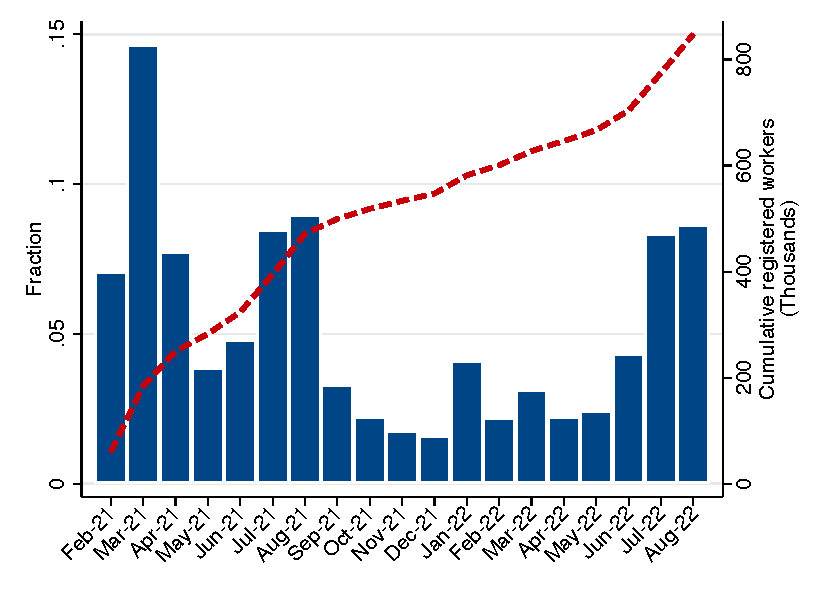
\includegraphics[width=0.65\textwidth]{04_Figures/muestra_1porciento/hist_download_month.pdf}
    \end{center}
\end{figure}
\scriptsize{
\noindent This figure shows the total number of workers registered for the RPCI. The right y-axis measures the fraction of workers who registered for the RPCI during each month from the total workers who registered for the RPCI. The left y-axis measures the cumulative number of workers who registered for the RPCI.
}

\clearpage

%\subsection{Event Studies: RPCI effect on enrollment and wages}

\begin{figure}[H]
    \centering
    \caption{Event studies - RPCI effect on enrollment and wages \label{fig:event_study_rpci}}
    
    \begin{subfigure}{0.49\textwidth}
    \caption{Effect on being enrolled}
    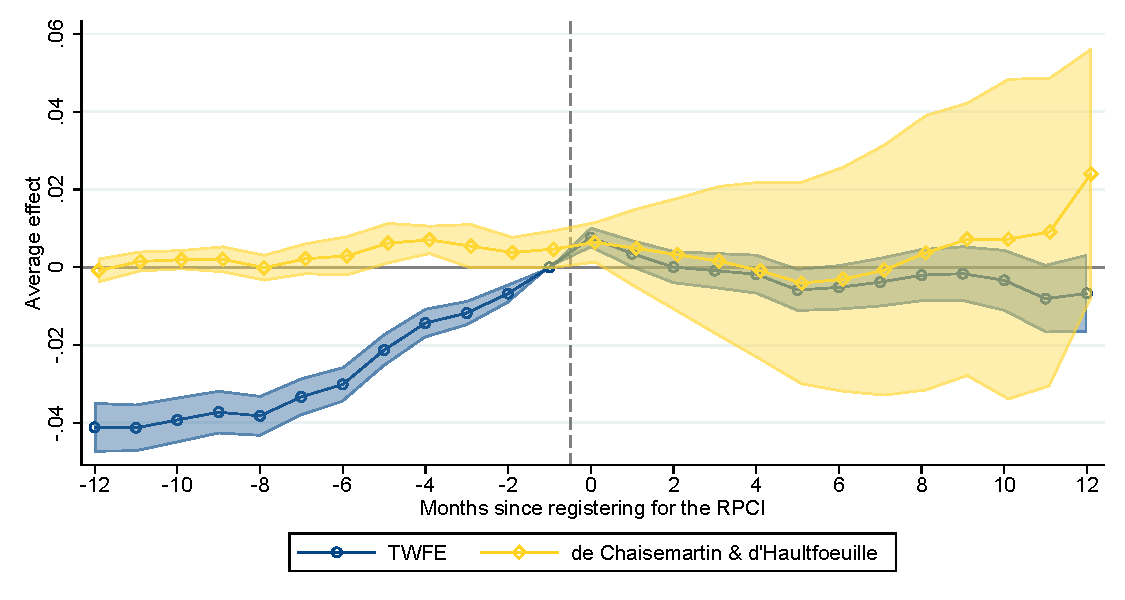
\includegraphics[width=\textwidth]{04_Figures/muestra_10porciento/event_study_alta_connected.pdf}
    \end{subfigure}
    \begin{subfigure}{0.49\textwidth}
    \caption{Effect on formal wage$^\dagger$}
    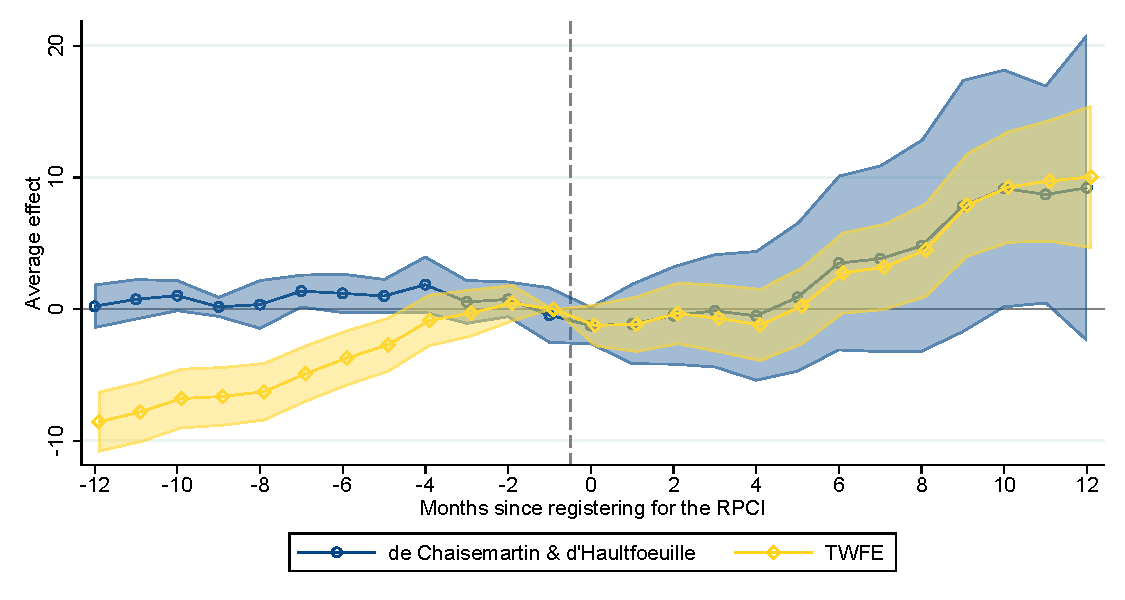
\includegraphics[width=\textwidth]{04_Figures/muestra_10porciento/event_study_sal_formal_connected.pdf}
    \end{subfigure}
    
    \begin{subfigure}{0.49\textwidth}
    \caption{Effect on wage}
    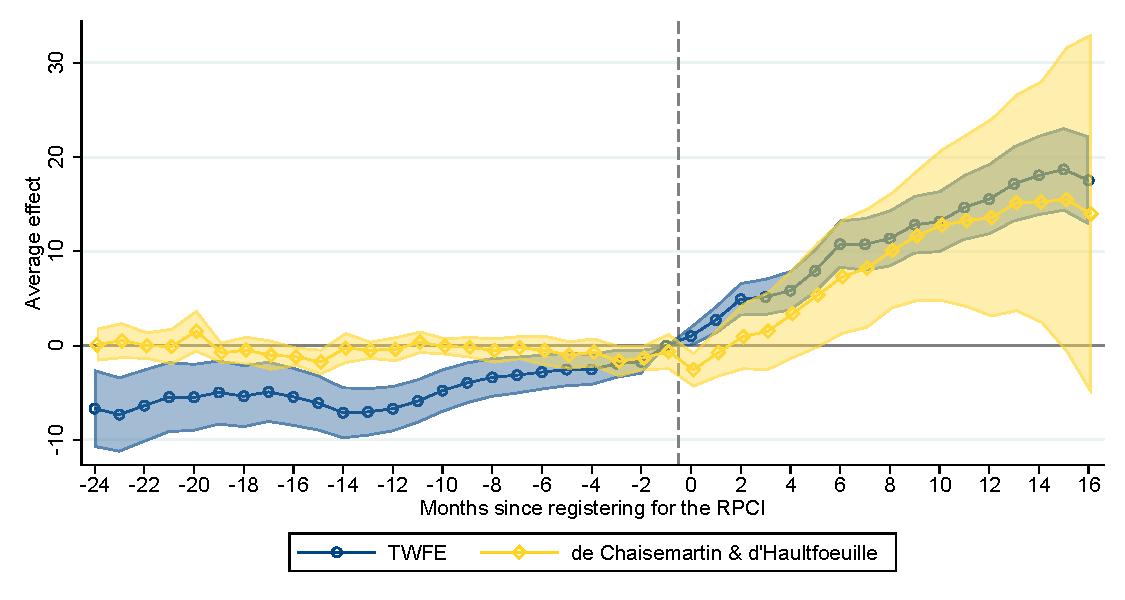
\includegraphics[width=\textwidth]{04_Figures/muestra_10porciento/event_study_sal_cierre_connected.pdf}
    \end{subfigure}
    \begin{subfigure}{0.49\textwidth}
    \caption{Effect on log wage}
    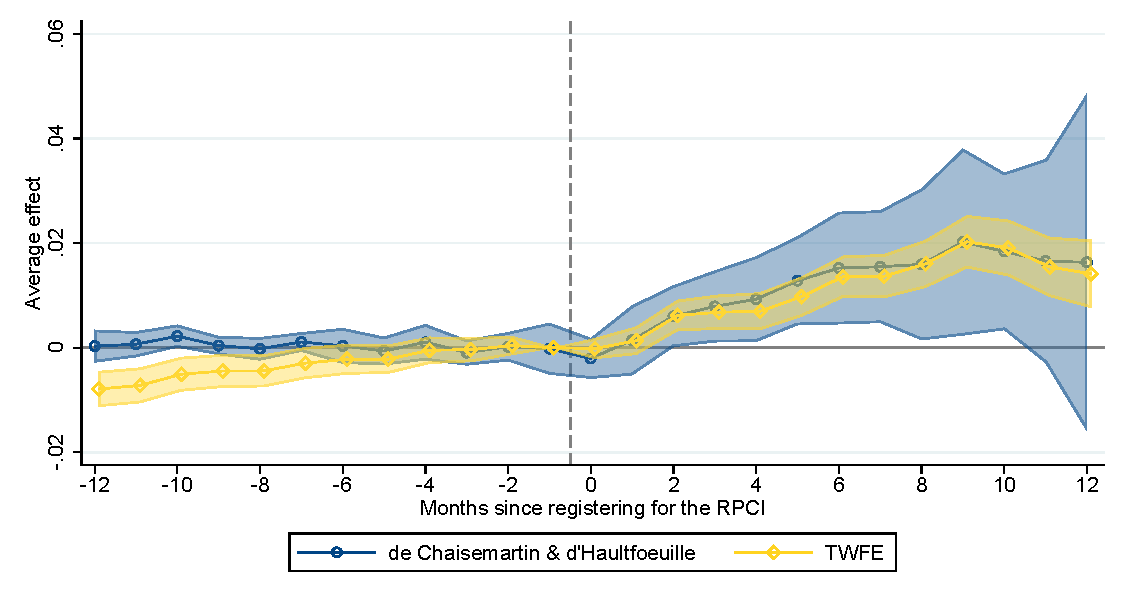
\includegraphics[width=\textwidth]{04_Figures/muestra_10porciento/event_study_log_sal_cierre_connected.pdf}
    \end{subfigure}
    
    %\textit{Do file: event_study_rpci.do}
\end{figure}

\scriptsize{
\noindent \textit{Notes}: This figure shows the event studies for the effect of registering to the RPCI on enrollment and the worker's wage. \textit{Sample:} Panel data for a random sample of the workers enrolled at the Mexican Institute of Social Security (IMSS) during 2020 and January 2021 (before the RPCI launch). \textit{Enrolled} is a dummy variable where 1 means worker $i$ was enrolled at IMSS during period $t$. $\dagger$ \textit{Formal Wage} and \textit{Wage} are the registered wage for worker $i$ during period $t$, the difference is \textit{Formal Wage} is 0 when the worker isn't enrolled, while \textit{Wage} is missing when the worker isn't enrolled. The lighter-shaded event studies present the estimators obtained from a TWFE specification. The darker-shaded event studies follow the estimators proposed by \cite{de2020two}, using the robust dynamic option to account for possible heterogeneous treatment effects across cohorts. Robust standard errors clustered by worker id. This figure is referenced in %\hyperref[subsec:workers]{Section} \ref{subsec:workers}.
}

\clearpage

\begin{comment}
    
%\subsection{Event Studies: RPCI effect on wage changes}

\begin{figure}[H]
    \centering
    \caption{Event studies - RPCI effect on wage changes \label{fig:event_study_wage_changes_rpci}}
    
    \begin{subfigure}{0.49\textwidth}
    \caption{Effect on wage changes}
    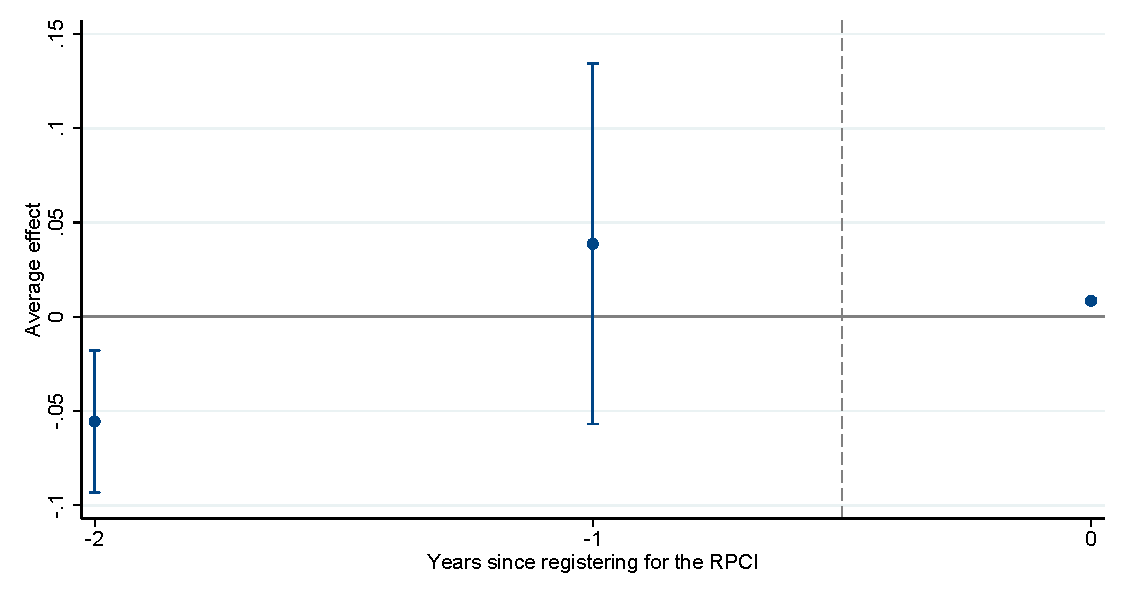
\includegraphics[width=\textwidth]{04_Figures/muestra_10porciento/event_study_sal_diff_yr_dcdh.pdf}
    \end{subfigure}
    
    \begin{subfigure}{0.49\textwidth}
    \caption{Effect on wage raises}
    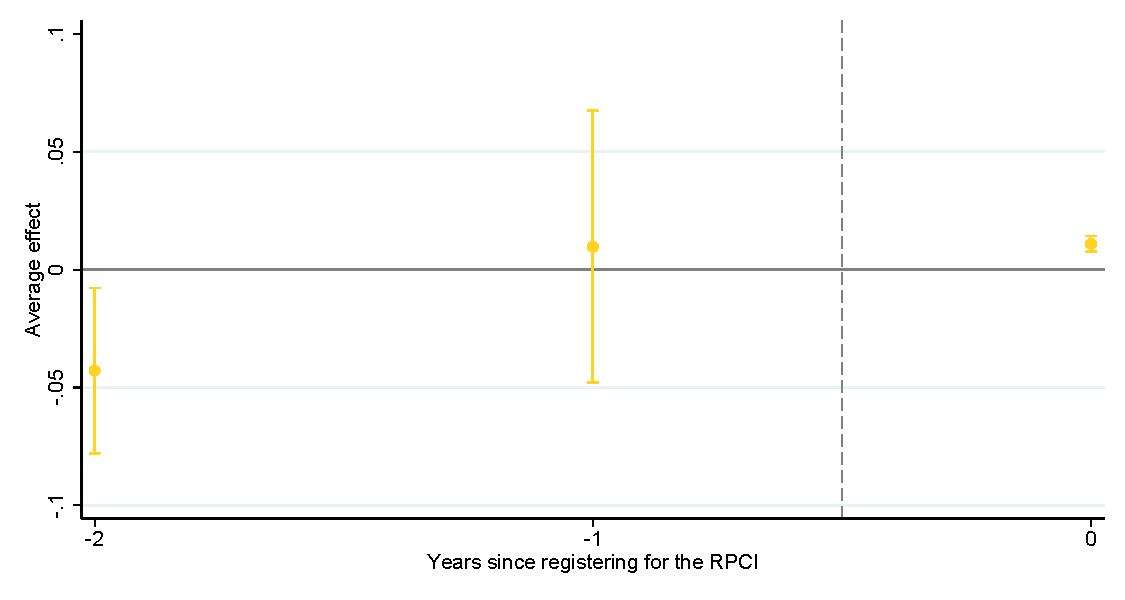
\includegraphics[width=\textwidth]{04_Figures/muestra_10porciento/event_study_sal_mayor_yr_dcdh.pdf}
    \end{subfigure}
    \begin{subfigure}{0.49\textwidth}
    \caption{Effect on wage cuts}
    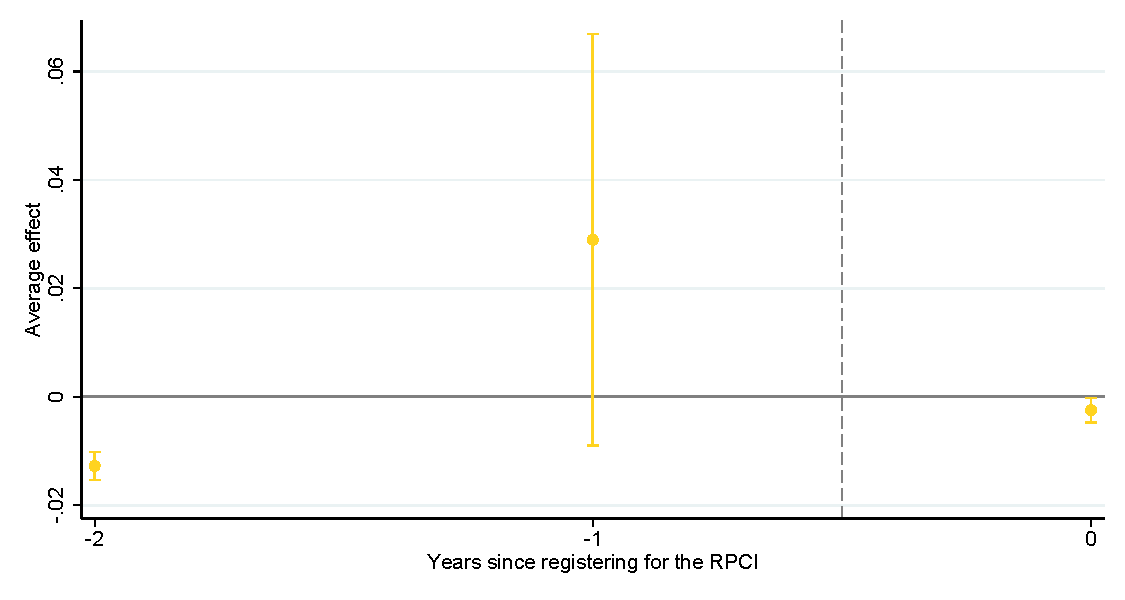
\includegraphics[width=\textwidth]{04_Figures/muestra_10porciento/event_study_sal_menor_yr_dcdh.pdf}
    \end{subfigure}
    
    %\textit{Do file: event_study_rpci.do}
\end{figure}

\scriptsize{
\noindent \textit{Notes}: This figures shows the event studies for the effect of registering to the RPCI on enrollment and the worker's wage. \textit{Sample:} Panel data for a random sample of the workers enrolled at the Mexican Institute of Social Security (IMSS) during during 2020 and January 2021 (before the RPCI launch). \textit{Wage Changes} counts the number of changes in the reported wage at IMSS of worker $i$ during year $t$. \textit{Wage Raises} counts the number of wage changes where the wage increased and \textit{Wage Cuts} counts the number of wage changes where the wage decreased. The event studies follow the estimators proposed by \cite{de2020two}, using the robust dynamic option to account for possible heterogeneous treatment effects across cohorts. Robust standard errors clustered by worker id. This figure is referenced in %\hyperref[subsec:workers]{Section} \ref{subsec:workers}.
}

%\subsection{Heterogeneity by worker characteristics}

\begin{figure}[H]
    \centering
    \caption{Heterogeneity by worker characteristics \label{fig:heterogeneity_worker_rpci}}
    
    \begin{subfigure}{\textwidth}
    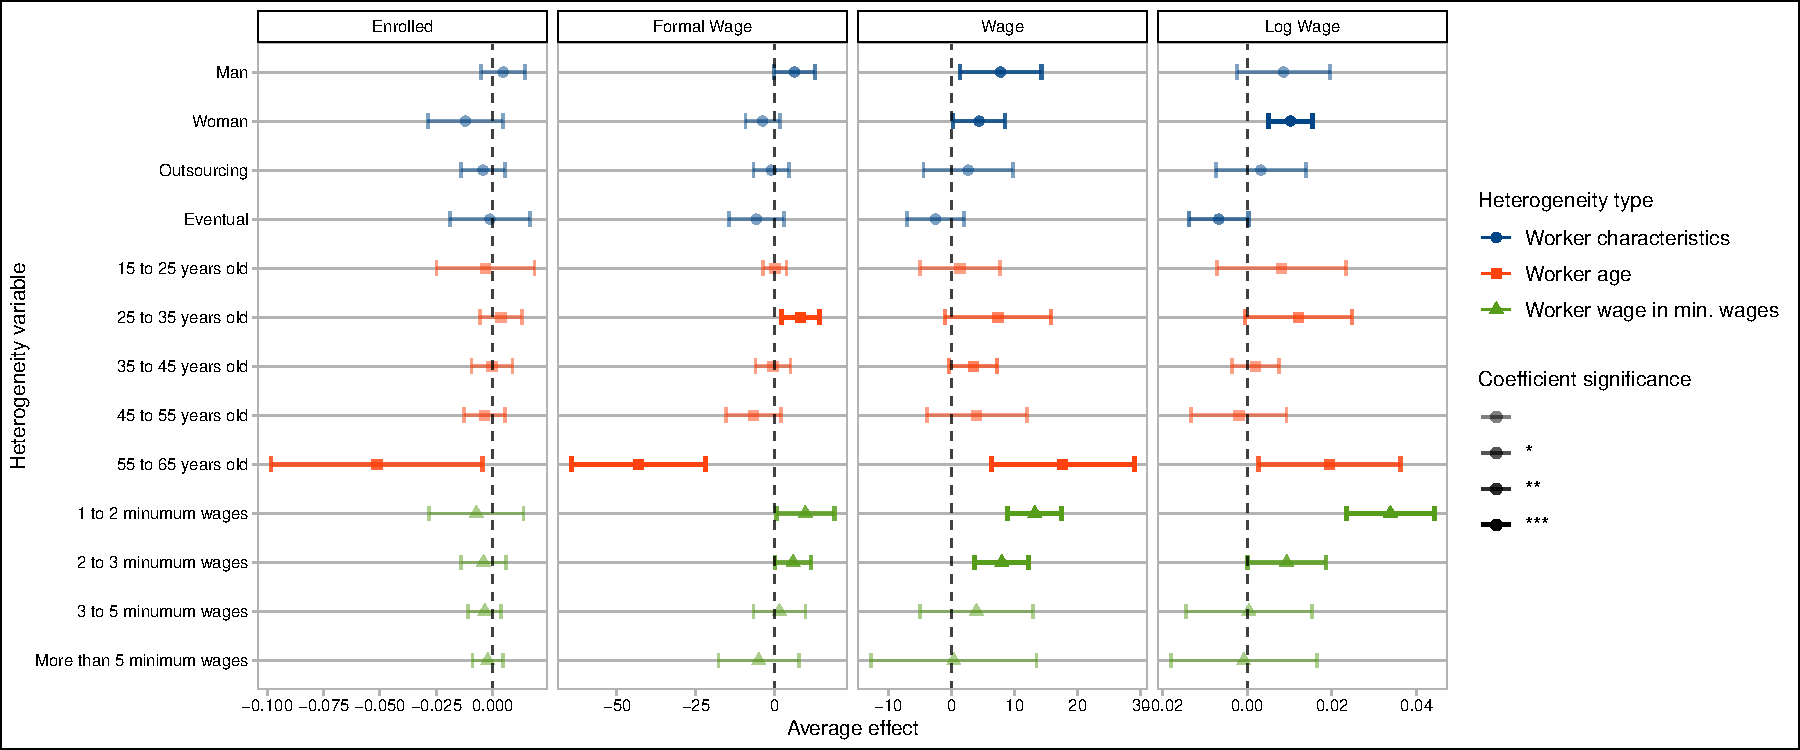
\includegraphics[width=\textwidth]{04_Figures/muestra_10porciento/dcdh_heterogeneity_worker_characteristics.pdf}
    \end{subfigure}
    
    %\textit{Do file: dcdh_heterogeneity_rpci.do}
\end{figure}

\scriptsize{
\noindent \textit{Notes}: This figure explores heterogeneity in the effect of registering to the RPCI on enrollment and the worker's wage by baseline worker's characteristics (characteristics during 2020, before the RPCI launch). \textit{Sample:} Panel data for a random sample of the workers enrolled at the Mexican Institute of Social Security (IMSS) during 2020 and January 2021 (before the RPCI launch). \textit{Enrolled} is a dummy variable where 1 means worker $i$ was enrolled at IMSS during period $t$. $\dagger$ \textit{Formal Wage} and \textit{Wage} are the registered wage for worker $i$ during period $t$, the difference is \textit{Formal Wage} is 0 when the worker isn't enrolled, while \textit{Wage} is missing when the worker isn't enrolled. The coefficient displayed is the average treatment effect estimated following \cite{de2020two}, using the robust dynamic option to account for possible heterogeneous treatment effects across cohorts. 95\% confidence intervals are shown. Robust standard errors clustered by worker id. *** $p<0.01$, ** $p<0.05$, * $p<0.1$. %This figure is referenced in %\hyperref[subsec:workers]{Section} \ref{subsec:workers}.
}

\clearpage

%\subsection{Heterogeneity by firm characteristics}

\begin{figure}[H]
    \centering
    \caption{Heterogeneity by firm characteristics \label{fig:heterogeneity_firm_rpci}}
    
    \begin{subfigure}{\textwidth}
    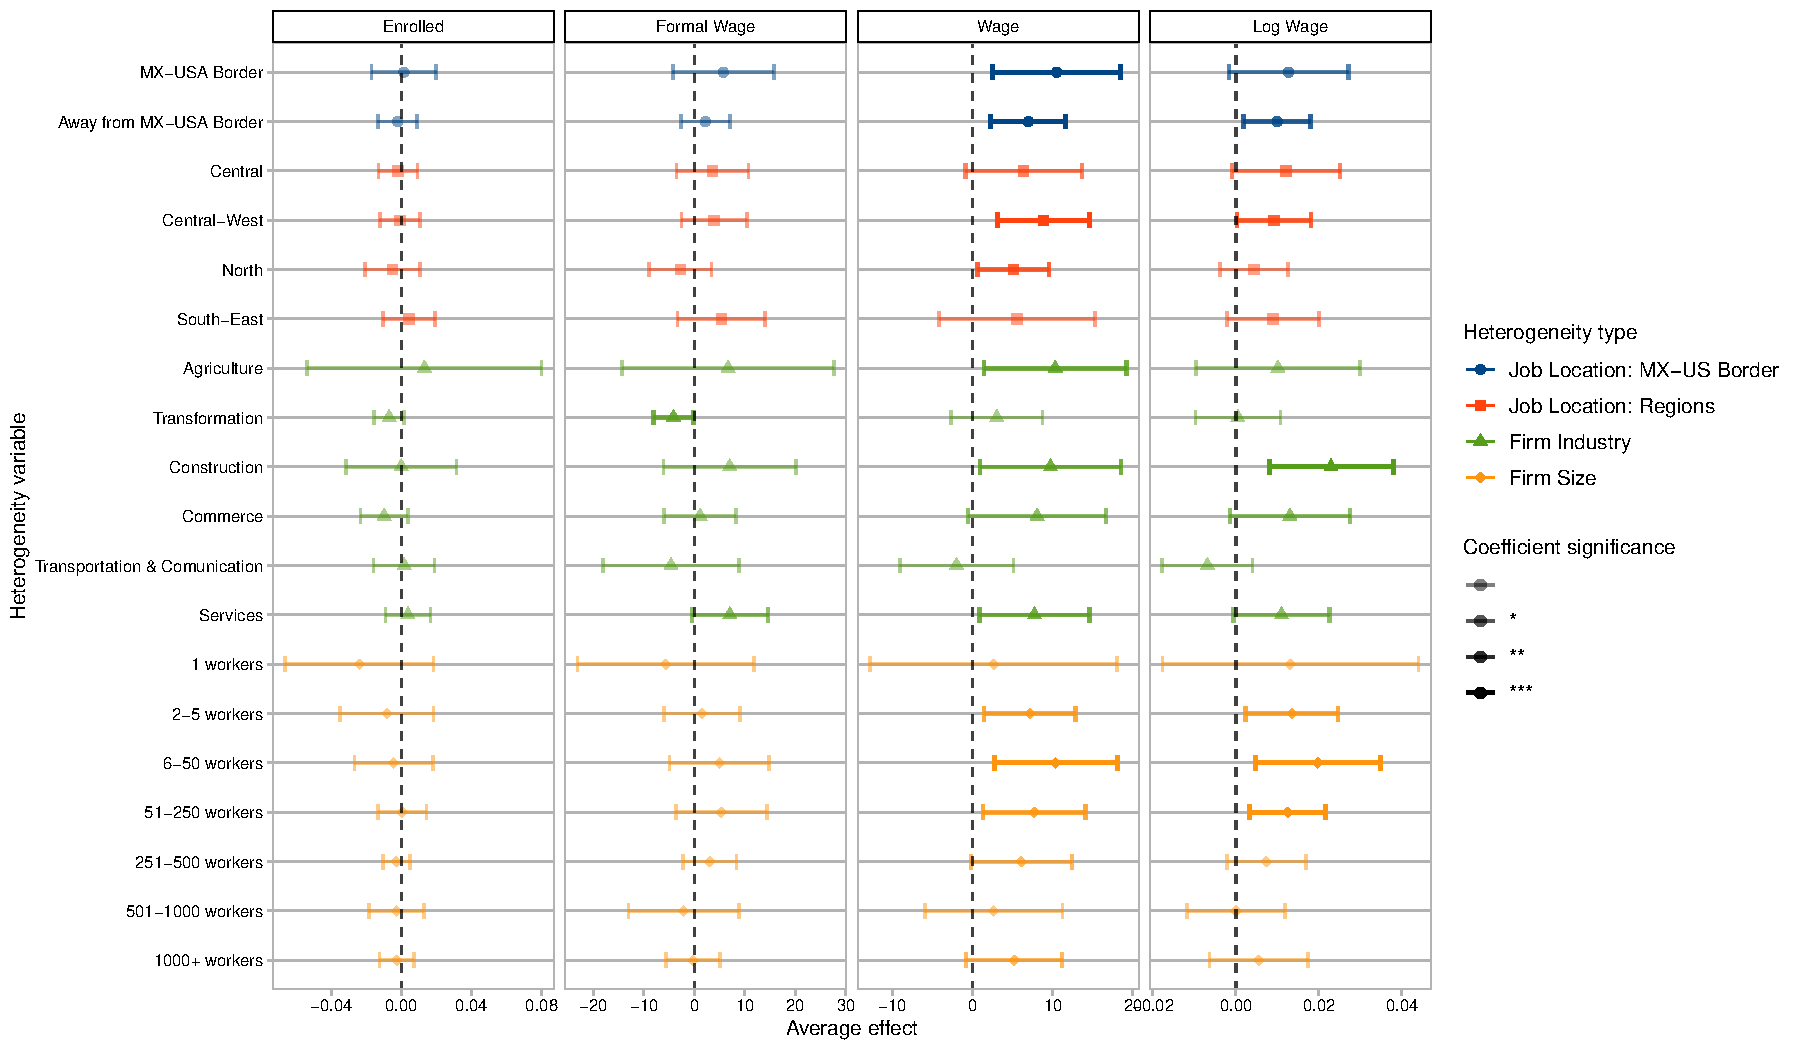
\includegraphics[width=\textwidth]{04_Figures/muestra_10porciento/dcdh_heterogeneity_firm_characteristics.pdf}
    \end{subfigure}
    
    %\textit{Do file: dcdh_heterogeneity_rpci.do}
\end{figure}

\scriptsize{
\noindent \textit{Notes}: This figure explores heterogeneity in the effect of registering to the RPCI on enrollment and the worker's wage by baseline firm's characteristics (characteristics during 2020, before the RPCI launch). \textit{Sample:} Panel data for a random sample of the workers enrolled at the Mexican Institute of Social Security (IMSS) during 2020 and January 2021 (before the RPCI launch). \textit{Enrolled} is a dummy variable where 1 means worker $i$ was enrolled at IMSS during period $t$. $\dagger$ \textit{Formal Wage} and \textit{Wage} are the registered wage for worker $i$ during period $t$, the difference is \textit{Formal Wage} is 0 when the worker isn't enrolled, while \textit{Wage} is missing when the worker isn't enrolled. The coefficient displayed is the average treatment effect estimated following \cite{de2020two}, using the robust dynamic option to account for possible heterogeneous treatment effects across cohorts. 95\% confidence intervals shown. Robust standard errors clustered by worker id. *** $p<0.01$, ** $p<0.05$, * $p<0.1$. This figure is referenced in %\hyperref[subsec:workers]{Section} \ref{subsec:workers}.
}

\clearpage

\end{comment}

%%%%%%%%%%%%%%%%%%%%%%%%%%%%%%%%%%%%%%%%%%%%%%%%%%%%%%

\newpage
%  \documentclass[oneside,11pt]{article}

% 
\usepackage{soul}
\usepackage{natbib}
\usepackage{hyperref}
\usepackage{bookmark}
\usepackage{graphicx}             
\graphicspath{{./Figuras/}}
\usepackage[dvipsnames]{xcolor}
\usepackage{todonotes}
\usepackage{makecell}
\usepackage[margin=1in]{geometry}
\usepackage{float}                
\usepackage{amsmath}
\usepackage{amscd}
\usepackage{amsfonts}
\usepackage{amssymb}
\usepackage{bbm}
\usepackage{booktabs}
\usepackage{nameref}
\usepackage{multirow}
\usepackage[nokeyprefix]{refstyle}
\usepackage{rotating}
\usepackage{threeparttable}
\usepackage{afterpage}
\usepackage{lscape}
\usepackage{enumerate}
\usepackage{caption}
\usepackage{subcaption}
\usepackage{epstopdf}
\usepackage{setspace}
\usepackage{svg}
\usepackage{dsfont}
\usepackage{amsthm}
\usepackage{tocloft}
\usepackage{etoc}
\usepackage{lmodern}
\usepackage{bm}
\usepackage[T1]{fontenc}
\usepackage{tgpagella}

\epstopdfDeclareGraphicsRule{.tiff}{png}{.png}{convert #1 \OutputFile}
\AppendGraphicsExtensions{.tiff}

\epstopdfDeclareGraphicsRule{.tif}{png}{.png}{convert #1 \OutputFile}
\AppendGraphicsExtensions{.tif}

\def\sym#1{\ifmmode^{#1}\else\(^{#1}\)\fi}

\usepackage{tikz}
\usetikzlibrary{shapes.geometric, arrows}
\usetikzlibrary{calc}
\usetikzlibrary{matrix}

\tikzset{ 
    table/.style={
        matrix of nodes,
        row sep=-\pgflinewidth,
        column sep=-\pgflinewidth,
        nodes={
            rectangle,
            draw=black,
            align=center
        },
        minimum height=1.5em,
        text depth=0.5ex,
        text height=2ex,
        nodes in empty cells,
%%
        every even row/.style={
            nodes={fill=gray!20}
        },
        column 1/.style={
            nodes={text width=2em,font=\bfseries}
        },
        row 1/.style={
            nodes={
                fill=black,
                text=white,
                font=\bfseries
            }
        }
    }
}


\usepackage{colortbl}
\usepackage{url}
\urlstyle{rm}
\definecolor{darkblue}{rgb}{0,0,.4}
\hypersetup{colorlinks=true, breaklinks=true, citecolor=Maroon, linkcolor=darkblue, menucolor=darkblue, urlcolor=darkblue}

\newtheorem{theorem}{Theorem}
\newtheorem{claim}[theorem]{Claim}
\newtheorem{prop}[theorem]{Proposition} 
\newtheorem{cor}[theorem]{Corollary} 
\newtheorem{assumption}{Assumption} 
\newtheorem{lem}{Lemma} 

\DeclareRobustCommand{\hlgr}[1]{{\sethlcolor{green}\hl{#1}}}


\usepackage{comment}
%para esconder columnas en tablas (enrique)
\usepackage{array}
\newcolumntype{H}{>{\setbox0=\hbox\bgroup}c<{\egroup}@{}}
\linespread{1.25}

\newcommand{\wh}{\widehat}
\usepackage{anyfontsize}

\usepackage[linesnumbered,vlined,ruled,commentsnumbered]{algorithm2e}

\DontPrintSemicolon
\newcommand{\To}{\mbox{\upshape\bfseries to}}
\newcommand{\E}{\mathbb{E}}

\DeclareCaptionFormat{cont}{#1 (cont.)#2#3\par}
% %%% HELPER CODE FOR DEALING WITH EXTERNAL REFERENCES
% \usepackage{xr}
% \makeatletter
% \newcommand*{\addFileDependency}[1]{
%   \typeout{(#1)}
%   \@addtofilelist{#1}
%   \IfFileExists{#1}{}{\typeout{No file #1.}}
% }
% \makeatother


% \newcommand*{\myexternaldocument}[1]{
%     \externaldocument{#1}
%     \addFileDependency{#1.tex}
%     \addFileDependency{#1.aux}
% }

% %\myexternaldocument{OA}

% %%%%%%%%%%%%%%%%%%%%%%%%%%%%%%%% DOCUMENT
% \begin{document}

%%%%%%%%%%%%%%%%%%%%%%%%%%%%%%%%%%%%%%%%%%%%%%%

% APPENDIX 
\setcounter{table}{0}
\setcounter{figure}{0}
\setcounter{section}{0}
\pagenumbering{gobble}


\begin{center}
	\LARGE IMSS RPCI \\[0.5em]
	\Large{Appendix $-$ For Online Publication} \\[1em]
	\large \author{Eduardo Alcaraz \and Gabriela López \and Luis Martínez \and Marco Medina \and Enrique Seira}
\end{center}

\appendix
\pagenumbering{arabic}
\renewcommand\thefigure{OA-\arabic{figure}}
\renewcommand\thetable{OA-\arabic{table}}
\renewcommand*{\thepage}{OA - \arabic{page}}
\renewcommand\thesection{Appendix \Alph{section}.}
\renewcommand\thesubsection{\Alph{section}.\arabic{subsection}}

%\renewcommand{\cftparskip}{0em} % NOT NEEDED
\renewcommand\cftsecdotsep{\cftdotsep}
\renewcommand\cftsubsecdotsep{\cftnodots}
\renewcommand{\cftsecnumwidth}{6em}
 \renewcommand{\cftpnumalign}{r}
%\renewcommand{\cftsecleader}{\normalfont\cftdotfill{\cftsecdotsep}}


\renewcommand{\cftsecleader}{\cftdotfill{\cftsecdotsep}\hspace{1.8em}}
%\renewcommand{\cftsecpagefont}{20em}
%\renewcommand{\cftfignumwidth}{6em}
%\renewcommand{\cfttabnumwidth}{3.3em}

%\tableofcontents
\etocdepthtag.toc{mtappendix}
\etocsettagdepth{mtchapter}{none}
\etocsettagdepth{mtappendix}{subsection}

\setstretch{0.9}
%\renewcommand\contentsname{} % the empty name

\begingroup
\let\clearpage\relax
%\vspace{-1.5em} % the removed space. Set as appropriate
\tableofcontents
\endgroup

\clearpage

\section{ RPCI}
\vspace{.2in}

\begin{figure}[H]
    \caption{RPCI flyers}
    \label{rpci_flyers}
    \begin{center}
    
    \begin{subfigure}{0.49\textwidth}
    \caption{RPCI flyer titled "Does my employer has me registered at IMSS?"}
    
\includegraphics[width=\textwidth]{04_Figures/rpci_app/rpci_flyer_3.jpeg}
    \end{subfigure}
    \begin{subfigure}{0.49\textwidth}
    \caption{RPCI flyer titled "Digital services for a healthy environment"}
    
\includegraphics[width=\textwidth]{04_Figures/rpci_app/rpci_flyer_2.jpeg}
    \end{subfigure}

    \end{center}
\end{figure}
\scriptsize{
\noindent Flyers circulated by the Mexican Institute of Social Security (IMSS) for the RPCI. Both flyers explain how you can track and access your job register information, such as wage and firm you are registered at, if you register for the RPCI.
}

\clearpage

\begin{figure}[H]
    \caption{Registering for the RPCI}
    \label{rpci_register}
    \begin{center}
    
    \begin{subfigure}{0.9\textwidth}
    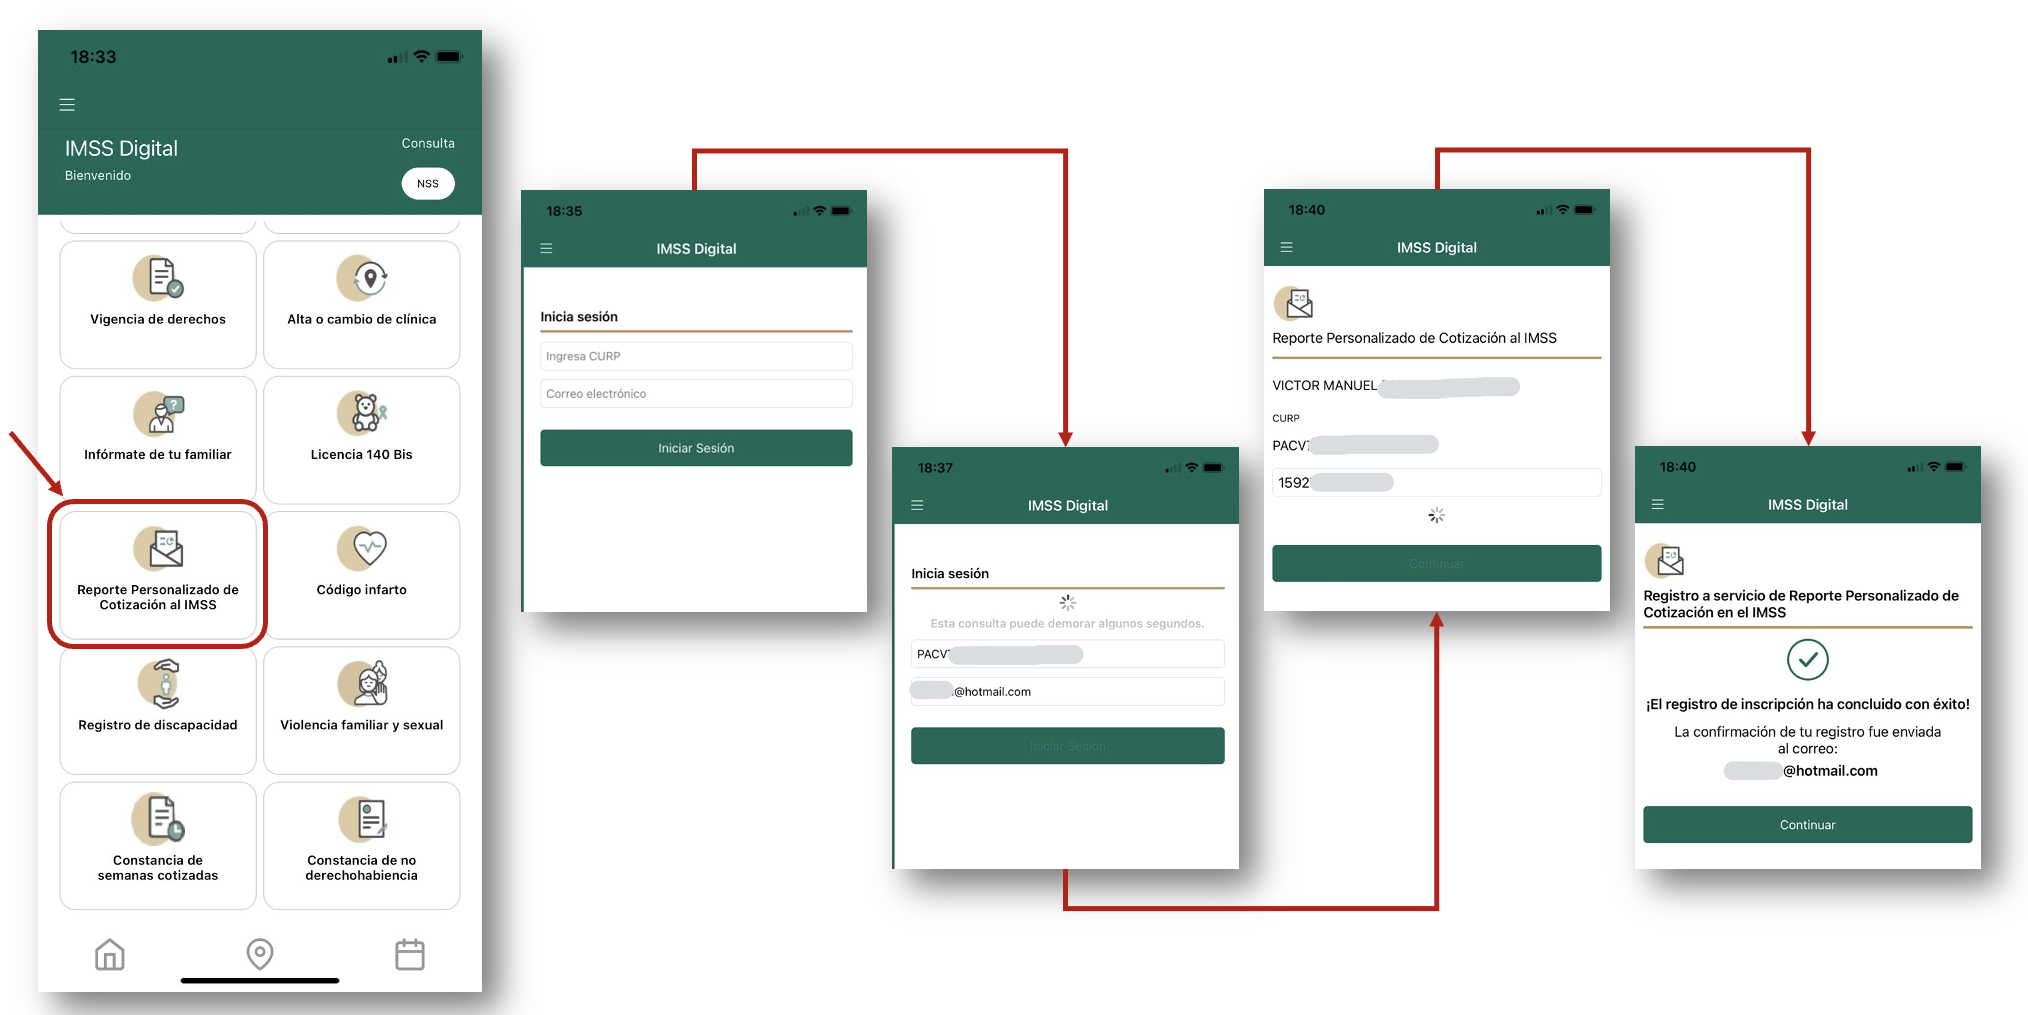
\includegraphics[width=\textwidth]{04_Figures/rpci_app/rpci_register.png}
    \end{subfigure}

    \end{center}
\end{figure}
\scriptsize{
\noindent Diagram shows how to register for the RPCI within the IMSS Digital app. The worker registers only once to access the RPCI, using his Unique Population Registry Key (CURP) and email address.
}

\clearpage

\begin{figure}[H]
    \caption{RPCI example}
    \label{rpci_example}
    \begin{center}
    
    \begin{subfigure}{0.49\textwidth}
    \caption{RPCI within the IMSS Digital app}
    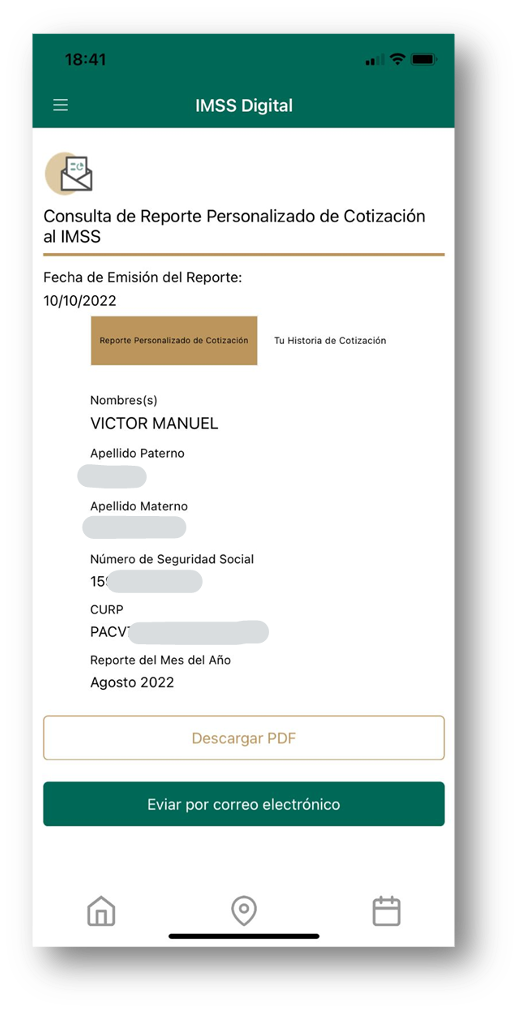
\includegraphics[width=\textwidth]{04_Figures/rpci_app/rpci_2.png}
    \end{subfigure}
    \begin{subfigure}{0.49\textwidth}
    \caption{RPCI PDF file}
    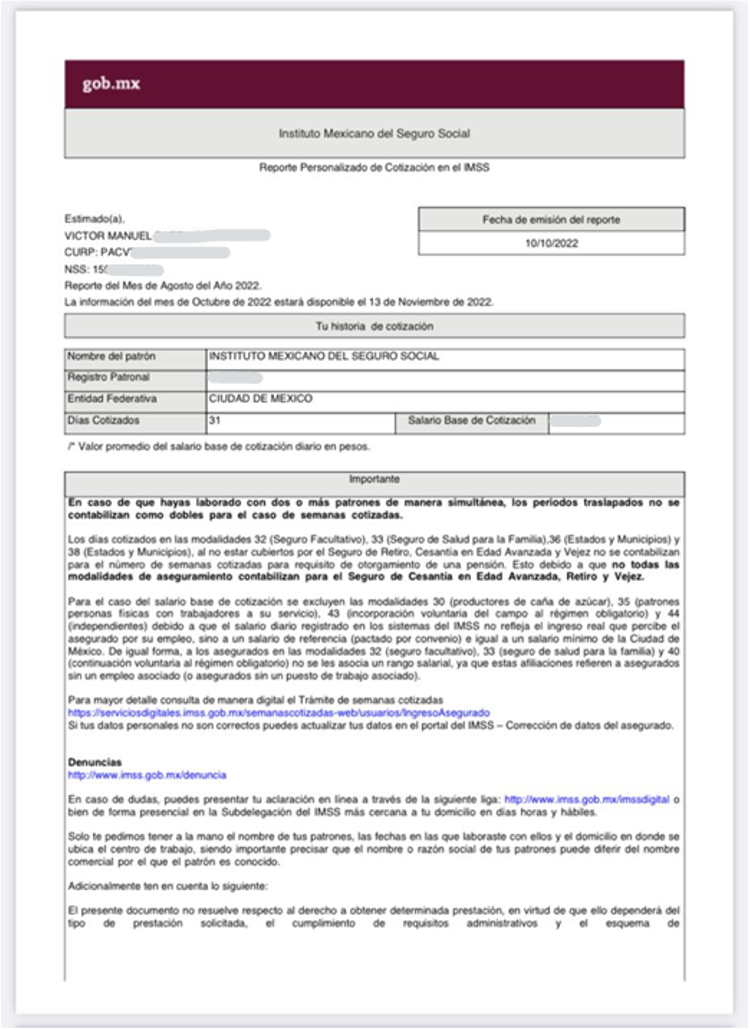
\includegraphics[width=\textwidth]{04_Figures/rpci_app/rpci_3.png}
    \end{subfigure}
    

    \end{center}
\end{figure}
\scriptsize{
\noindent Figure (a) shows the IMSS Digital app, where once the worker is registered for the RPCI, the worker can download their report in PDF or receive it via email. Figure (b) shows an example of the PDF for the RPCI. The report includes the worker job registered information, such as wage and the firm the worker is registered at.
}

%\clearpage

%\bibliographystyle{authordate1}
%\bibliographystyle{amsalpha}
%\bibliographystyle{AER}

%\bibliography{References}




% \end{document}

\end{document}

